%% To submit your paper:
\documentclass[draft]{agujournal2019}
\usepackage{url} %this package should fix any errors with URLs in refs.
\usepackage{lineno}
\usepackage[inline]{trackchanges} %for better track changes. finalnew option will compile document with changes incorporated.
\usepackage{soul}
\linenumbers
\usepackage{multirow}
\usepackage{amsmath}
\usepackage{amssymb}
\usepackage{siunitx}
\usepackage{booktabs}
\usepackage{xr}
\usepackage{xspace}

\hfuzz=100pt
\hbadness=10000

\externaldocument{supplement}  % no .tex extension

\draftfalse

\journalname{JGR: Atmospheres}

%%%%%%% MAKE SOME COMMANDS %%%%%%%%%%
\newcommand{\eqtn}[1]{Eq.~(\ref{#1})}       % Equation reference
\newcommand{\fig}[2]{\textcolor{red}{(Fig.~\ref{#1}{#2})}}   % Figure reference
\newcommand{\fignop}[2]{\textcolor{red}{Fig.~\ref{#1}{#2}}}  % Figure reference

\newcommand{\todo}[1]{\textcolor{purple}{TODO: #1}}      % Comments
\newcommand{\comment}[1]{\textcolor{cyan}{#1}}     % TODO notes
\newcommand{\mynum}[1]{\textcolor{olive}{#1}}

% meteorological terms go here
\newcommand{\tmin}{\textcolor{black}{$T_{\mathrm{min}}$}\xspace}
\newcommand{\tair}{\textcolor{black}{$T_{\mathrm{air}}$}\xspace}
\newcommand{\tsfc}{\textcolor{black}{$T_{\mathrm{sfc}}$}\xspace}
\newcommand{\qair}{\textcolor{black}{$q_{\mathrm{air}}$}\xspace}
\newcommand{\qsfc}{\textcolor{black}{$q_{\mathrm{sfc}}$}\xspace}
\newcommand{\lwnet}{\textcolor{black}{$LW_{\mathrm{net}}$}\xspace}
\newcommand{\wspd}{\textcolor{black}{$w_{\mathrm{spd}}$}\xspace}
\newcommand{\wdir}{\textcolor{black}{$w_{\mathrm{dir}}$}\xspace}
\newcommand{\cloudfrac}{\textcolor{black}{$C_{\mathrm{frac}}$}\xspace}
\newcommand{\dq}{\textcolor{black}{$\Delta q$}\xspace}
\newcommand{\dT}{\textcolor{black}{$\Delta T$}\xspace}
\newcommand{\fq}{\textcolor{black}{$F\mathrm{_q}$}\xspace}
\newcommand{\ustar}{\textcolor{black}{$u_{\star}$}\xspace}
\newcommand{\lwup}{\textcolor{black}{$LW^{\uparrow}$}\xspace}
\newcommand{\lwdn}{\textcolor{black}{$LW^{\downarrow}$}\xspace}
\newcommand{\tsnow}{\textcolor{black}{$T_{\mathrm{snow}}$}\xspace}
\newcommand{\qsnow}{\textcolor{black}{$q_{\mathrm{snow}}$}\xspace}
\newcommand{\pbaro}{\textcolor{black}{$P_{\mathrm{baro}}$}\xspace}
\newcommand{\rnet}{\textcolor{black}{$R_{\mathrm{net}}$}\xspace}
\newcommand{\hs}{\textcolor{black}{H$_s$}\xspace}
\newcommand{\hlat}{\textcolor{black}{H$_l$}\xspace}
\newcommand{\swnet}{\textcolor{black}{$SW_{\mathrm{net}}$}\xspace}
\newcommand{\swdn}{\textcolor{black}{$SW^{\downarrow}$}\xspace}
\newcommand{\swup}{\textcolor{black}{$SW^{\uparrow}$}\xspace}
\newcommand{\dcc}{\textcolor{black}{$\Delta$CC}\xspace}
\newcommand{\albedo}{\textcolor{black}{$\alpha$}\xspace}
\newcommand{\rfalb}{\textcolor{black}{RF$_{albedo}$}\xspace}
\newcommand{\rfcirrus}{\textcolor{black}{RE$_{cloud}$}\xspace}
\newcommand{\rfcanopy}{\textcolor{black}{RF$_{canopy}$}\xspace}
\newcommand{\dswe}{\textcolor{black}{$\Delta$SWE}\xspace}


% units
\newcommand{\um}{\textcolor{olive}{$\mu$m}\xspace}
\newcommand{\ms}{\textcolor{olive}{m$\cdot$s$^{-1}$}\xspace}
\newcommand{\gkg}{\textcolor{olive}{g$\cdot$kg$^{-1}$}\xspace}
\newcommand{\kmsq}{\textcolor{olive}{km$^2$}\xspace}  % kilometers
\newcommand{\wmsq}{\textcolor{olive}{W$\cdot$m$^{-2}$}\xspace}
\newcommand{\degr}{\textcolor{olive}{$^\circ$}\xspace}
\newcommand{\degrc}{\textcolor{olive}{$^\circ$C}\xspace}
\newcommand{\gmtwo}{\textcolor{olive}{gm$^{-2}$}\xspace}
\newcommand{\kgmtwo}{\textcolor{olive}{kg$\cdot$m$^{-2}$}\xspace}
\newcommand{\mjmtwo}{\textcolor{olive}{MJ$\cdot$m$^{-2}$}\xspace}


\begin{document}


\title{Solar radiation primarily drives snow ablation during the March 2026 heat wave in the California Sierra Nevada}



\authors{William Rudisill\affil{1}, Alan Rhoades\affil{1}, Megan Mason\affil{2}, Gabriel Lewis\affil{2}, Andrew Schwartz\affil{2}, Marianne Cowherd\affil{4}, Benjamin Hatchett\affil{3}, Erica Siirila-Woodburn\affil{1}, Dan Feldman\affil{1}}

\affiliation{1}{Lawrence Berkeley National Laboratory, Earth and Environmental Sciences Area}
\affiliation{2}{UC Berkeley Central Sierra Snow Laboratory}
\affiliation{3}{Colorado State University}
\affiliation{4}{Montana State University}
%(repeat as many times as is necessary)

\correspondingauthor{William Rudisill}{williamrudisill@lbl.gov}

\begin{keypoints}
% \item A record heat wave led to record rates of snow ablation during March 2026 in the California Sierra Nevada. 
\item March 2026 in the central California Sierra Nevada was the warmest on record, exceeding previous record set during the 1934 Dust Bowl. 
\item Net-shortwave radiation was the dominant driver of record rates of snow ablation for both forest and open sites. 
\item Less than \mynum{1}\% of total snow ablation was due to sublimation in the open, lower than the climatological average for March.

% these are not included in the three key points 
\item Surface layer stability and vapor pressure arguments explain the small contribution of sublimation to the snow energy and mass balance during the heat wave.
\item Sub-canopy snow was more directly temperature sensitive due to longwave effects, but the canopy ultimately inhibited energy exchange to the snow during the heat wave.

\end{keypoints}

\begin{abstract}
It is generally accepted that solar radiation is the most important snow-ablation forcing, but this poses a paradox: why are ``snow-eater heat waves'' so effective at ablating snow? 
Using the 3-$\sigma$ heat wave of March 2026 observed at the Central Sierra Snow Laboratory in the California Sierra Nevada (2100 m.a.s.l) as a case study, we ask the following questions: What are the energy balance mechanisms influencing ablation during the heat wave? 
Does vegetation canopy enhance or suppress rates of ablation? 
How much snow melts versus sublimates?
We find the record snow ablation rates remain dominated by solar radiation and snow-albedo decline.
In addition to extreme warmth, March 2026 was also the sunniest in the CERES satellite record (+\mynum{42} \wmsq above average).
Canopy cover increases the longwave radiation absorbed by sub-canopy snow, but solar shading and reduced turbulent exchange yields lower ablation rates under canopy (\mynum{-18} mm/day) compared to the open site (\mynum{-25} mm/day). 
Despite anomalously low snowpack cold content prior to the heat wave, sensitivity tests show a minimal influence of the starting state of the snowpack on the rate of snow ablation.
Sublimation (less than \mynum{1}\% of total snow ablation in the open) was a relatively minor factor during the heat wave. 
Theoretical arguments show that atmospheric buoyancy effects and vapor pressure gradient limitations explain the limited role of evapo-sublimation during heat waves. 
Future synoptic-scale analyses of snow--heat wave interactions should focus on the covariance of heat wave conditions, wind speed, and atmospheric thermodynamic conditions that lead to prolonged cloud-free conditions.

\end{abstract}



\section{Introduction}
While meltwater from seasonal snowpacks has historically provided $\sim$70\% of runoff in the western US (WUS) \cite{Li2017-dj}, these natural reservoirs and our ability to accurately measure, monitor, and predict them are in decline \cite{Hale2023-kx, Cowherd2024-zm}.
From a practical perspective, many operational snowmelt runoff models use a temperature index approach, whereby air temperature (\tair) is the primary predictor of melt \cite{Anderson1973-jx}.
While these models have proven effective, especially for large basins and when well-calibrated \cite{REIS-model}, the physical justification for such models is not clear.
Since at least the 1980s, the field of snow hydrology has appreciated that understanding the climatic behavior of snow necessitates considering the entire energy budget of the snowpack.
In particular, it is well accepted that the net shortwave radiation absorbed by the snowpack (\swnet) is a first-order predictor of rates of melt \cite{Marks1992-qo, Cline1997-de}.
Both small impurities \cite{Deems2013-vv, Skiles2018-ih} and wet and dry grain-growth mechanisms \cite{Colbeck1982-gv} tend to decrease the amount of reflected sunlight (the snow albedo, \albedo) and are responsible, in conjunction with rising sun-angles, for the large increases in springtime \swnet into mid-latitude snowpacks.
Unlike downwelling longwave (\lwdn; 4--100 \um), the downwelling component of shortwave (\swdn; 0.3--3 \um) is mainly insensitive to variations in \tair itself.
Variations in \swdn in time (and across elevation) are driven primarily by Rayleigh scattering by O$_2$ and N$_2$, Mie scattering by naturally occurring and human-made aerosols, dust, and cloud droplets, as well as absorption primarily by water vapor, CO$_2$, and O$_3$.

% recent heat wave work
At the same time, recent work has highlighted the strong correlation between extreme snow ablation (the loss of snow to either sublimation or melt) events and so-called ``snow-eater heat waves'' (SEHW) --- prolonged periods of sustained, anomalous, and above-freezing \tair during the snow season \cite{Rhoades2026-jm}.
The characteristics of snow-eater heat waves have already appreciably changed since the 1850s, and these events are occurring more frequently, at a higher intensity, over a larger portion of the WUS, and earlier in the water year.

%These with warming in addition to the mean-annual air temperature.
An example of such an early-season, high-intensity, SEHW occurred in March of 2026, when the monthly March \tair across the WUS was 3-$\sigma$ above long-term averages.
This event (which started earlier than the window of occurrence studied in \citeA{Rhoades2026-jm}) resulted in widespread and rapid ablation at many snow-observing sites \cite{Marshall2026-sy}, and streamflow that was one-to-two months earlier than average in many watersheds (e.g., \fignop{fig:supp_sagehen_q}{}).
This ablation raises an apparent paradox: if \swdn provides most of the energy for snowmelt, and yet it is largely insensitive to \tair, then why are heat waves so efficient at ablating snow?

% It has been argued that their efficacy arises not from the relationship between \tair and turbulent fluxes of sensible heat into the snowpack, but rather the relationship between longwave radiation (\lwdn) emitted by the atmosphere \citep{Pluss1997-wx, Ohmura2001-ll}.
% % \cite{Brutsaert1975-jl} showed that \todo{the radiative transfer equations reduce to .... }.

% what are we going to do
Using the March 2026 event as a case study, we ask the following questions:
\begin{itemize}
  \item What are the dominant snow ablation energy forcings during spring heat waves, and how do they scale with increasing \tair?
  \item How do vegetation canopies and atmospheric conditions --- including clouds or lack thereof --- shape such energetic forcings during heat wave events and the rate of snow ablation?
  \item What are the relative contributions of sublimation and melt to extreme snow ablation during such events?
\end{itemize}

% why we should care about veg
Approximately one-third of North America's snow water volume resides in forests \cite{Kim2021-eu}.
Previous work shows the dominant influence of forest on sub-canopy snow arises from the balance between solar shading and longwave emission from trees, which tend to have a higher emissivity than the clear-sky atmosphere \cite{Sicart2004-kf}, and for this reason sub-canopy snow dynamics are sensitive to latitude (insofar as it controls \swdn) and mean winter \tair (insofar as it is related to \lwdn) \cite{Lundquist2013-uc}.  
Several studies have considered the effects of vegetation on the mean-state of the snow climate in the Sierra Nevada \cite{Harpold2020-rc, Krogh2020-dh, Piske2025-qi} which tend to show that, like other regions of the WUS mountains, forest reduces snow duration relative to adjacent open areas \cite{Lundquist2013-uc}.
However, in terms of rate of melt, forests may enhance melt rate (relative to open areas) during the mid-winter when the sun is weak \cite{Bales2011-vs}, while reducing melt rates during the spring \cite{Kittredge1953-iy}.
Therefore, it is not clear whether the ablation rate of sub-canopy snow should increase or decrease relative to open areas during early spring SEHW conditions. 

% clouds
Despite otherwise drier-than-normal conditions, high-altitude cirrus clouds can occur during high-pressure ridging events commonly associated with cool-season heat waves (\citeA{Rhoades2026-jm} Figure 1 and Supplemental Figure S5). 
Dry, sinking air associated with high-pressure ridges may also preclude the formation of low or mid-level clouds, which have the largest impact on the snow energy balance \cite{Rudisill2025-cx} and are generally associated with reduced rates of snow ablation and streamflow \cite{Sumargo2018-zf}.
Frameworks for investigating interactions between clouds and surface radiation are well explored in the literature, using satellite retrievals and surface radiation data \cite{Ramanathan1989-pa, Shupe2004-kl, L-Ecuyer2019-my}, but little work has investigated the extent to which clouds, or the lack thereof (e.g., \citeA{McEvoy2023}), contribute to anomalous snow ablation in mid-latitude regions.

% outcomes
The outcomes from this study answer basic science questions about energy available for snowmelt or sublimation in water-resource-critical basins in the Sierra Nevada, with implications for other regions.
The findings can directly inform efforts towards management and resilience against extreme events by providing actionable steps towards improving the monitoring and prediction of snowmelt and provide considerations for forest management efforts \cite{Harpold2020-rc}.
Lastly, improved understanding of vegetation and snow interactions during heat waves can inform headwater management practices through improved decision support tools (e.g., \citeA{Heggli2026}).


\section{Background and Methods}


\subsection{Study area}\label{sec:study_area}
Our study is focused on observations collected at the Central Sierra Snow Laboratory (CSSL; 39.32 $^\circ$N, 120.37 $^\circ$W, 2100 m.a.s.l) located in Soda Springs, CA \cite{Schwartz_Cowherd_McGurk_Mason_Riker-Coleman_Zutter_Lewis_2026} in the central California Sierra Nevada \fig{fig:region_map}{a--e}.
In order to contextualize the regional-scale characteristics of the March 2026 snow drought and associated mechanisms, we also evaluate snow and \tair anomalies across the surrounding 
South Yuba, North Fork American, and Truckee River Watersheds.
The Yuba and North Fork American rivers support the New Bullards Bar and Folsom reservoirs, respectively, both of which are managed for flood risk reduction and longer-term storage.
All three watersheds support varied downstream consumptive uses (i.e., urban, industrial and agricultural) and provide critical aquatic and riparian habitats.


\subsection{Observational data}\label{sec:observational_data}
\subsubsection{Snow and near-surface data}
% snotel and USHCRN
We use data from twelve Natural Resources Conservation Service (NRCS) SNOwpack TELemetry (SNOTEL) Network stations located throughout the study region \fig{fig:region_map}{b} spanning 1905 to 2605 m.a.s.l.
SNOTEL is the primary snow observing program in the WUS \cite{Serreze1999-as} and routinely measures snow water equivalent (SWE), precipitation, and \tair, though the homogeneity of \tair measurements remains a challenge for the SNOTEL network \cite{Oyler2015-by, McAfee2019-mt}.
To supplement SNOTEL temperature records, we use data from four US Historical Climatology Network (USHCN) stations and the gridded nClimGrid \cite{Durre2022-be} throughout the study region.
USHCN stations are a high-quality subset of the larger GHCN-D dataset \cite{Menne2012-uu}.
The HCNv2 dataset provides homogenized and quality-assured monthly \tair based on USHCN data that dates as far back as the late 1800s \cite{Menne2009-ushcn}.
While these data do not have the same spatial density and elevation range as SNOTEL, the longer temporal record and high quality control mean that these observations can more confidently be used for evaluation of climate extremes, such as heat wave events \cite{BercosHickey2022}.

% csssl
In addition to hosting an NRCS SNOTEL site, CSSL provides long-term meteorological and snowpack records as well as surface energy balance measurements.
Campbell Scientific CNR4 four-component radiometers measure incoming ($\downarrow$) and outgoing ($\uparrow$) SW and LW radiation from the atmosphere and snowpack.
A Campbell Scientific IRGASON eddy covariance system measures sensible (H$_s$) and latent (H$_l$) heat fluxes above the snowpack.
The CSSL forest study site hosts an additional meteorological station approximately 130 m north of the main CSSL site.
This tower hosts an additional Kipp and Zonen SP Lite2 radiometer that measures below-canopy SW radiation.
SWE measurements were obtained using a federal sampler \cite{Osterhuber2014-ic} at nine discrete sampling intervals during the March heat wave in the forest location.

% ranking SWE anomalies
To rank or contextualize SWE anomalies, we use the framework from \citeA{Hatchett2022}, which uses a percentile-based metric to assign snow drought categories.
Drought categories are ranked as abnormally dry (D0), moderate drought (D1), severe drought (D2), extreme drought (D3), and exceptional drought (D4) for values between the 30th--20th, 20th--10th, 10th--5th, and 5th--2nd percentiles, and below the 2nd percentile, respectively.
SWE percentiles are computed using the NRCS SNOTEL periods of record for each site.
Z-scores are used to rank near-surface \tair and snow ablation anomalies.
Baseline mean and standard deviations are computed using a common 30-year 1981--2010 normal period following NOAA standards, unless otherwise stated.
Other deviations from normal conditions are expressed as the ``anomaly,'' which is the difference between the current state and the sample mean.



% Both the IRGASON and CNR4 are hosted on a movable arm \fig{fig:region_map}{c} that automatically adjusts to maintain a constant distance of approximately one meter above the snow surface as snow accumulates or ablates throughout the season.

\subsubsection{Atmospheric data}
% era5 and other data
To investigate the atmospheric dynamics associated with the March heat wave, we use 500 hPa geopotential height and atmospheric column information from the fifth-generation ECMWF Reanalysis (ERA5) \cite{Hersbach2020-era5}.
Daily geopotential height anomalies during the event are computed using data provided by \citeA{Lee2023-cc}.
Heights have been de-trended and cover the period from 1979 to 2022.

% radiation
We use the Clouds and the Earth's Radiant Energy System (CERES) Energy Balanced and Filled (EBAF), hereafter CERES-EBAF \cite{Kato2018-pi}, to investigate the effects of clouds, or lack thereof, on the snow energy balance.
CERES-EBAF provides gold-standard measurements of monthly surface and top-of-atmosphere (TOA) irradiances at a 1$^\circ\times$1$^\circ$ resolution.
This product is suitable for trend analysis.
While coarse in resolution, the lower-level hourly products have demonstrated good performance when evaluated against in-situ radiometers in mountains collected by intensive field campaigns \cite{Rudisill2025-cx, Feldman2023-gp} and when used directly as forcings for snow simulations \cite{Hinkelman2015-ri}.
The 2000--present period-of-record of CERES-EBAF is used to examine the March anomaly in \swdn and \lwdn and the contribution of clouds to the anomalies therein.
CERES-EBAF provides all-sky and clear-sky estimates of downwelling surface radiative fluxes which are used to estimate cloud radiative effect (\rfcirrus; described in a subsequent section). 

%  and CERES-SYN1Deg \cite{Rutan2015-ar},
% CERES-SYN1Deg is a lower-level product that provides hourly estimates of the same quantities but is not configured to examine long-term temporal trends.
% Thus, we use CERES-SYN1Deg all-sky and clear-sky \swdn and \lwdn (e.g., hypothetical irradiance in the absence of clouds) to compute cloud-radiative effects following \citeA{Ramanathan1989-pa} and subsequent studies.

\subsection{SUMMA model configuration}\label{sec:models:summa}
\subsubsection{Model details}
Neglecting precipitation related terms, the energy budget of a snowpack is given by:
\begin{align}\label{eq:energy_budget}
\mathrm{Melt}/ \mathrm{Refreeze}  - \Delta\mathrm{CC}
&= 
\underbrace{
    H_\mathrm{s} + H_\mathrm{l}
}_{\text{turbulent fluxes}}
+
\underbrace{
LW\downarrow- \sigma\epsilon T_{snow}^4
}_{\text{net longwave}}
+
\underbrace{
   SW\downarrow(1-\alpha)
}_{\text{net shortwave}}
+
G,
\end{align}
where the left-hand side represents changes in the internal state of the snowpack and the right-hand side represents fluxes at the top/bottom of the snow control volume. 
Melt/Refreeze is the rate of melt or liquid water refreezing in mass per second multiplied by the latent heat of fusion, $\Delta$CC is the time rate-of-change in the snowpack cold content (CC; \citeA{Jennings2018-wz}), $H_s$ and $H_l$ are the turbulent fluxes of sensible and latent heat respectively at the snow/atmosphere interface, \tair is the temperature of the air, \tsnow is the temperature of the snow surface, $\epsilon$ is the emissivity of the snow (0.98), \swdn is the downwelling shortwave radiation, and $\alpha$ is the albedo of the snow surface defined as the ratio of upwelling shortwave radiation (\swup) to \swdn.
CC is signed such that it is by definition always equal to (in the case of isothermal, 0\degrc snow) or less than zero.
Sign conventions are such that positive terms represent energy directed into the snowpack or snow melting, and negative the opposite (refreezing).

% summa
We use the process-based Structure for Unifying Multiple Modeling Alternatives (SUMMA) v3.3.0 model \cite{Clark2015-ni} configured at a point scale to solve Eq. \ref{eq:energy_budget} for open and forested conditions.
SUMMA is well-vetted for a range of snow climate applications and provides several options for flux stability corrections, canopy radiation interactions, snow-layering schemes, and other model structural options \cite{Cristea2022-ys}.
We use the Jordan snow layering option, which allows for up to 100 snow layers, the ``Louisinv'' option for stability correction of turbulent fluxes, and the ``stickySnow'' canopy snow interception scheme.
We assign a measurement height of 12 m for the model forcings into SUMMA in order to intercompare the effects of 10 m tall needleleaf vegetation characteristic of the forest site at CSSL using the same forcing variables.

% albedo
Snow albedo (\albedo) is computed with SUMMA's ``varDecay'' parameterization, in which visible and near-infrared albedos are prognostic and evolve as a balance between refreshment by snowfall and decay by grain growth, which is accelerated exponentially as the top snow layer temperature rises, and further accelerated by a ``slush'' term near the melting point, plus a constant rate impurity loading. 

%% what does vegetation do
Vegetation canopy influences the snow energy balance in SUMMA through several mechanisms.
We use the ``UEB-2stream'' approximation for canopy radiation interactions.
An LAI value of 1.5 was assigned based on data from nearby representative regions \cite{Krogh2020-dh}.
These choices are further validated by comparing modeled sub-canopy \swdn for a range of LAI values against the CSSL radiometers in the forest site, and finding good agreement \fig{fig:supp_sw_validation}{}.
The incident \lwdn to the sub-canopy snowpack is modeled as the sum of \lwdn unobscured by the vegetation, weighted by $(1-\varepsilon_c)$, plus a component emitted by the canopy, weighted by the canopy emissivity $\varepsilon_c$.
SUMMA solves for a vegetation energy balance and canopy air-space temperature which is used in the LW emission calculation.
In SUMMA, $\varepsilon_c$ is purely a function of the leaf-area index (LAI) and stem-area index.
We turn off vegetation phenology in the model such that $\varepsilon_c$ is constant for these experiments.

% more data
\subsubsection{Model forcings}
We use hourly ERA5 data \cite{Hersbach2020-era5} as SUMMA model forcings after bias correcting the data to observations at CSSL.
Daily precipitation from the NRCS SNOTEL site is used directly as forcing when available, assuming a constant hourly precipitation rate within each day, in place of the ERA5 precipitation rate.
Hourly ERA5 two-meter \tair are bias corrected to match the monthly average \tair observed at the CSSL from the NRCS records by removing a constant linear bias term.
ERA5 \swdn data are adjusted to match the CNR4 data by applying a \swdn correction coefficient as a function of the solar zenith and azimuth angles to adjust the ERA5 data to account for shadows (see \fignop{fig:supp_fig_SWd_adjust_sza_azm}{}).
To ensure that the ERA5 data matches the best available estimates of variability and trends in radiation at this site, we use a multiplicative scale that forces the ERA5 \swdn and \lwdn monthly anomalies to match monthly anomalies in the CERES-EBAF data.
Other forcing variables compared favorably against the available observations and were not adjusted.
Additional information about SUMMA validation is provided in the Supplemental Material (Sec.~\ref{supp:sec:validation}).



\subsubsection{Model evaluation and sensitivity testing}\label{sec:methods:radforce}
To aid in the interpretation of changes in the snow energy balance, we apply the radiative forcing concept in several ways in this study \cite{Ramanathan1989-pa, Deems2013-vv, Rudisill2025-cx}.
In this context, radiative forcing quantifies the instantaneous difference in the net, or in a single stream, of radiation between observed conditions and a counterfactual reference state (Table \ref{tab:radiative_effects}).

% clouds
We define RF$_{canopy}$ as the difference between \rnet under the canopy and \rnet outside of the canopy layer.
Lacking observations sufficient to constrain RF$_{canopy}$, we use the SUMMA model to evaluate this quantity and express this value for both LW and SW components.
To investigate the relative contribution of \albedo decay to the surface radiation balance, we quantify the \albedo radiative forcing (\rfalb) by differencing \swnet computed using observed \albedo versus \swnet computed using observed \swdn and a hypothetical fresh-snow broadband \albedo; for this work we use 0.85, which is slightly lower than that used in similar work (e.g., \citeA{Gibson2026-zk}).

We define a cloud radiative ``effect'', rather than ``forcing'', to express the influence of clouds on downwelling \lwdn and \swdn terms only (\rfcirrus), since a full accounting of cloud radiative effects on net-energy terms also depends on the amount of reflected and absorbed energy by the surface, and therefore the snow \albedo \cite{Rudisill2025-cx} and assumptions about varying upwelling emissions.
All radiative effects are signed such that positive indicates energy is added to the snowpack via that process (clouds, canopy, or \albedo decay), and a negative sign indicates the opposite.

\begin{table}[h]
\centering
\caption{Definitions of radiative effect (the difference in downwelling terms only) and forcing (the difference in net-radiation) used in this study.
All effects are signed positive when energy is added to the snowpack.
$x$ refers to the radiative component, which is either SW, LW, or the sum of SW and LW.}
\label{tab:radiative_effects}
\begin{tabular}{lll}
\hline
\textbf{Name} & \textbf{Abbreviation} & \textbf{Equation} \\
\hline
Cloud Radiative Effect          & RE$_{cloud}$      & F$_\text{x, cloudy}\downarrow$  - F$_\text{x, clear}\downarrow$ \\
Canopy Radiative Forcing        & RF$_{canopy}$     & F$_\text{x, under-canopy}$     - F$_\text{x, open}$ \\
Albedo Radiative Forcing        & RF$_{albedo}$     & \swdn[(1-$\alpha_\text{obs}$)  - (1-$\alpha_\text{clean}$)]\\
\hline
\end{tabular}
\end{table}


% initial condition experiments
In addition to running SUMMA for historical conditions, we also run sensitivity tests to isolate the effects of individual forcings and initial conditions on snow ablation during March 2026. 
The specifics of these experiments are described in subsequent sections.
Additional specific modeling parameterizations with relevance to this study are described in the Supplemental Material (Sec.~\ref{supp:summa_desc_model_eq}).
Table \ref{tab:definitions} lists commonly used abbreviations in this study.


\section{Results}

\subsection{The March 2026 SEHW}
% how hot was it
A four-station composite of the long-term and homogenized monthly USHCN HCNv2 data shows that 2026 had the highest March \tair observed since 1910, and was over 5 $^\circ$C above the 1981--2010 average --- greater than 3-$\sigma$ above the mean \fig{fig:ushcn_data}{a}.
The previous record for March average \tair was the 1934 Dust-bowl \cite{Cook2014-ba} for each of the four stations in the composite. 
The nClimGrid likewise shows a +5--8 $^\circ$C anomaly above average across the domain \fig{fig:ushcn_data}{b}.
This prolonged period of heat resulted from an extreme and persistent ridge of high pressure that gained strength throughout March \fig{fig:era5_anoms}{a}, with 500 hPa geopotential height anomalies exceeding 2-$\sigma$ (\mynum{200} m) in many circumstances. 

% stuff b4 the heat
The region experienced three notable periods of weather immediately prior to the March 2026 heat wave \fig{fig:era5_anoms}{b,c}. 
While the water-year-to-date precipitation (1 October--28 February) was nearly 100\% of normal leading up to March 2026 (not shown), there was a prolonged mid-winter dry spell \cite{Hatchett2023} from 7 January to 9 February during which SWE began ablating \fig{fig:era5_anoms}{c}.
Then, between 14--19 February, a total of 100 mm of new SWE accumulated at CSSL.
This snowfall event was followed by anomalously warm \tair and a rain-on-snow (ROS) event on the 24--25 of February that brought 91 mm of rainfall, leading to a net decline in SWE \fig{fig:era5_anoms}{b,c}. %overall stoke levels of the shred community also abruptly declined as well.

% synoptic pattern of the heat wave
March began with average to slightly above average \tair.
As the high-pressure ridge grew over the WUS, daily maximum \tair peaked at \mynum{20}\degrc on 20 March at CSSL but remained well above normal from 8--31 March, with daily \tair values at the Tahoe City USHCN station yielding anomalies of 2-$\sigma$ or greater for four days between the 17th--27th.
SEHW conditions meeting the \citeA{Rhoades2026-jm} criteria were met for over a two-week period between \mynum{11} and \mynum{26} March.
SEHW conditions were also met in the latter few days of February following the ROS event.

Correspondingly, the 500 hPa geopotential height anomaly exceeded 200 meters across the WUS on 16 March, and was greater than 2-$\sigma$ above the detrended mean for that date.
The hemispheric wave pattern on this day is characteristic of an amplified North American Dipole pattern \cite{Wang2014,Wang2015,Singh2016-ev}.

% how does the snow melt
Snow began ablating consistently starting with the February ROS event for both the open and forest sites and continued into the month of March.
We find good agreement between both SUMMA and observed SWE \fig{fig:era5_anoms}{c} and rates of ablation.
SWE ablated at an average rate of \mynum{-9.4} mm/day (\mynum{-8.2} mm/day) between 1--14 March, after which it accelerated to a rate of \mynum{-24.9} mm/day (\mynum{-17.7} mm/day) until the end of the month in the open (forest), ablating completely in the open by the \mynum{28th} and in the forest site by the \mynum{25th}.
Modeling results also show that, starting on 1 March, the snow contained significant liquid water throughout the depth of the pack on the order of 1--2\% by volume due to the antecedent ROS event.
A small snowfall event occurred on 1--2 March, and another occurred at the end of the month, on the 31st.


%%%%%%%%%%%%%%%%%%%%%%%%%%%%%%%%%%%%%%
% Snow water equivalent anomalies
%%%%%%%%%%%%%%%%%%%%%%%%%%%%%%%%%%%%%%
\subsection{SWE anomalies during water year 2026}\label{sec:swe_anomalies}

% how much swe melted
SWE ablated completely earlier, and at a faster rate than is typical for March, at SNOTELs throughout the study region \fig{fig:swechange}{a--c}.
The beginning of March saw SWE at ``None'', D0, or D1 drought levels across the twelve SNOTEL sites \fig{fig:swechange}{d}.
While SWE was nearly 0 mm for two of the lower-elevation sites (station ID numbers 473 and 809), this was not particularly anomalous for those locations on this date.
By the end of March, 9 of the 12 stations reached 0 mm SWE and the remaining sites were in a D3 (``extreme drought'') drought classification \fig{fig:swechange}{e}.
Only 4 of the SNOTEL sites had a precedent for 0 mm of SWE on 31 March.
Similarly, the snow-covered area reached its lowest ever recorded value on 31 March during the Moderate Resolution Imaging Spectroradiometer (MODIS) record (see Supplemental Material; \fignop{fig:supp_scachange}{}).
These findings are consistent with the observation that, WUS-wide, 17\% of SNOTELs had the lowest mid-March SWE on record \cite{Marshall2026-sy}.

% snow melt in context of the climate
An important distinction, however, is that the rate of monthly snow ablation (\dswe) was also anomalous at most sites \fig{fig:swechange}{f}.
Typically, most SNOTEL sites in this region gain (or remain constant) rather than lose SWE throughout March \fig{fig:swechange}{f} with the exception of the two lowest elevation sites.
Nine out of 12 sites, including CSSL, measured their highest rate of monthly SWE ablation for the SNOTEL record.
Two of the lowest elevation sites (473, 809) did not have anomalous \dswe in part because the starting value was so close to zero \fig{fig:swechange}{d}.
%%%%%%%%%%%%%%%%%%%%%%%%%%%%%%%%%%%%%%
% ENERGY BALANCE PLOTS
%%%%%%%%%%%%%%%%%%%%%%%%%%%%%%%%%%%%%%

\subsection{The snow energy balance in the open and forest site}
Having examined the geographic and climatic context of March 2026 snow ablation (Sec. \ref{sec:swe_anomalies}) we can begin to investigate the causes of anomalous ablation, which are fundamentally governed by the energy balance of the snow (Eq. \ref{eq:energy_budget}). 
To do so, we now focus on the CSSL site (site ID 428 in \fignop{fig:swechange}{} and also depicted in \fignop{fig:era5_anoms}{c}).
We examine time series of energy balance components (Eq. \ref{eq:energy_budget}) by separating them into nighttime, daytime, and 24-hour averages (\fignop{fig:open_seb}{a--f}, \fignop{fig:forest_seb}{a--f}).

% turb
\hs and \hlat are relatively minor factors compared to radiative fluxes (\fignop{fig:open_seb}{a,b}, \fignop{fig:forest_seb}{a,b}).
A period of significant sublimation occurred (negative \hlat) from 5--7 March, which corresponds with relatively high wind speed \fig{fig:era5_anoms}{c} but prior to the onset of the March SEHW conditions.
Another significant sublimation event took place on 24 March.
The highest rates of \hs occurred between 3--10 March and again between 21--26 March.
A maximum daytime \hs exceeding \mynum{80} \wmsq took place on 23 March for both the forest and open sites, three days after the peak of March \tair.

% shortwave and longwave
\swnet, however, far exceeds the \hs maxima in the open site (\fignop{fig:open_seb}{c}, \fignop{fig:forest_seb}{c}), and exceeds \mynum{240} \wmsq by the end of the month (with 24 hr averages of approximately \mynum{120} \wmsq).
Rates are significantly lower in the forest.
\swnet increases throughout March, but never exceeds \mynum{80} \wmsq in the forest site.

% lwnet
In the forest, \lwnet is positive on average for the entire month except the period spanning 4--7 March, which also corresponds with the only period of significant overnight CC production (\fignop{fig:open_seb}{d}, \fignop{fig:forest_seb}{d}).
Overnight \lwnet switches from slight negative ($\approx$ \mynum{-8} \wmsq) to positive or near-zero by 16 March in the forest site.
The highest rate of \lwnet occurs on 22 March, two days after the \tair peak of the heat wave event, and exceeds \mynum{60} \wmsq during the daytime.

\lwnet in the open site is of the opposite sign. 
This means the snow is continuously losing heat via longwave emission, even during the peak of the heat wave in the latter half of March, and on the order of \mynum{-80} to \mynum{-40} \wmsq \fig{fig:open_seb}{d}.

% melt and cc
The preceding energy exchanges, in addition to ground heat flux (not shown), cumulatively manifest as energy directed towards breaking/reforming ice crystalline bonds (Melt/Refreeze) and warming ice to the melting point (\dcc).
A significant amount of energy is added back to the snowpack during the nighttime by liquid water refreezing (\mynum{-6 to -33} \wmsq) in the open site, and to a lesser extent in the forest site (\fignop{fig:open_seb}{e}, \fignop{fig:forest_seb}{e}).
The overnight \lwnet cooling in the open yields overnight \dcc that is eroded the following day, prior to the initiation of melt (yielding net-zero averages over a 24 hour period; \fignop{fig:open_seb}{f}).
The cumulative overnight production in CC becomes small compared to the following day's melt by 14 March and represents less than \mynum{20}\% of the total melt energy, indicating that the lack of overnight CC production --- almost purely driven by the decline in \lwnet and increase in overnight \hs --- yields a snowpack that is primed for ablation the following day in the open site.

The dynamics of \dcc are different in the forest --- there is a near-zero amount of overnight CC production and very little refreezing.
These model results are confirmed by morning field reports from CSSL observers, who found melt-refreeze crusts in the open during March but slush in the forest site.


\subsection{Radiative forcing by canopy and snow aging}
The radiative forcing concept (Sec. \ref{sec:methods:radforce}) can be used to further interpret daily and monthly variation in the energy fluxes described previously, and shed light on the differences between the open and forest site energy balance mechanisms \fig{fig:radiative_forcing}{a--f}.

% albedo
Both \rfalb and \rfcanopy have a demonstrable impact on the energy balance.
The broadband snow \albedo started at a relatively low value leading up to the March heat wave (\mynum{0.6} to \mynum{0.7}) and declines consistently following a small refresh from the snowfall event on the first of the month \fig{fig:radiative_forcing}{a}.
The declines are well-matched by remote sensing and CSSL observations \fig{fig:supp_albedo_validation}{}.

% rf albedo
\rfalb increases at the open site as a function of rising sun-angle, \swdn (not shown), and \albedo decline, reaching a value approaching \mynum{92} \wmsq in the open site based on the SUMMA simulation.
While there is only a minor difference in the SUMMA model snow \albedo between the forest and open sites, \rfalb in the open exceeds \rfalb in the forest site by more than a factor of four by the end of the heat wave due to attenuation of \swdn by the canopy layer \fig{fig:radiative_forcing}{b}.

% canopy
Second in terms of magnitude to \rfalb, \rfcanopy yields a \mynum{+30} to \mynum{-30} \wmsq maximum daily rate during the month \fig{fig:radiative_forcing}{c}.
There are two competing effects that govern the net effect of canopy on the snow energy balance. 
\rfcanopy$_{,LW}$ increases as a function of \tair at a rate of \mynum{3.3} \wmsq per \degrc of (daily-average) \tair, which is visualized by considering the daily relationship for the entire SUMMA output record for the month of March \fig{fig:radiative_forcing}{e}.
Additional analysis (not shown) indicates that the canopy temperature is consistently warmer than the ambient \tair during the daytime, which, combined with the canopy emissivity relationship described in Sec. \ref{sec:models:summa}, explains this effect.
However, \rfcanopy$_{,LW}$ does not perfectly mirror \tair during March, which likely results from the energy balance of the canopy layer and also variations in atmospheric \lwdn emission.

This effect does not exceed the shading effect of the canopy (\rfcanopy$_{,SW}$), however, because the canopy attenuates much of the incident sunlight, so \rfcanopy$_{,Net}$ is near-zero and transitions to negative (cooling the snow) during the hottest part of the heat wave when the sun is also the most intense and the \albedo is at its lowest.

% total amounts
Ultimately, the cumulative energy transmitted from the atmosphere to the snow attributed to \rfalb is \mynum{+152} and \mynum{+32} \mjmtwo for the open and forest sites respectively, and \rfcanopy is responsible for a \mynum{-5.4} \mjmtwo effect (reducing energy incident on the snowpack).
\rfcirrus is evaluated in Sec. \ref{sec:results_ceres_ebaf}.


% \rfcirrus (SW) has a value of \mynum{-49} \mjmtwo and \rfcirrus (LW) has a value of \mynum{+31} \mjmtwo cumulatively.
% A full accounting of the net-effect of \rfcirrus on the snow energy balance also requires taking into account what is reflected and absorbed by the snow.
% Assuming a weighted albedo value of 0.6 (and that the CERES-SYN1Deg data is applicable at this scale) a coarse estimate of the net-cloud radiative forcing yields \mynum{+11} \mjmtwo of heating to the snow in the open \fig{fig:radiative_forcing}{f}.


%%%%%%%%%%%%%%%%%%%%%%%%%%%%%%%%%%%%%%
% ENERGY BALANCE PLOTS
%%%%%%%%%%%%%%%%%%%%%%%%%%%%%%%%%%%%%%
\subsection{Climatological context of the March 2026 snow energy balance}\label{sec:climo_comparison}
%
How does the March 2026 energy balance compare to typical Marches at CSSL?
As we have seen previously, SWE typically accumulates rather than ablates \fig{fig:swechange}{f} during the month of March.
We caution that this is not equivalent to saying that Melt does not occur, since snow may retain liquid water up to its residual saturation prior to the initiation of outflow.
We compute cumulative sums, in \mjmtwo, of the different energy balance terms to quantify their total contributions to ablation (\fignop{fig:monthly_seb_mar}{a--f} and Table \ref{tab:forest_open_summary}); for reference, 1 \mjmtwo of energy is equivalent to approximately \mynum{3.0} mm of snowmelt or \mynum{0.35} mm of snow sublimation. 
Sums are computed only for times when snow is present on the ground during March 2026 (\mynum{28 days} in the open and \mynum{25 days} in the forest). 
The same time periods are used for the historical period for fair comparison.


% the results
\swnet is both the strongest forcing (\mynum{+229.3} \mjmtwo) and also the most anomalous forcing compared to the 2000--present March average (\mynum{+120.3} \mjmtwo), followed by $H_s$ (\mynum{+39.7} \mjmtwo, with a \mynum{+17} anomaly) in the open site (\fignop{fig:monthly_seb_mar}{a}, Table \ref{tab:forest_open_summary}).
For the forest site, \swnet is also the strongest forcing (\mynum{+52.1} \mjmtwo) but not the most anomalous.
The most anomalous forcing in the forest is \lwnet, which is the second strongest forcing (\mynum{+28.1} \mjmtwo).
For a typical year, \lwnet is below zero (and a source of snow cooling) rather than a source of energy for heating snow under canopy.

% the snow albedo 
The weighted-average snow $\bar{\alpha}$ during March (computed as the monthly sum of \swup over the monthly sum of \swdn) is more than 1-$\sigma$ below the historical mean at both the open and forest sites \fignop{fig:monthly_seb_mar}{c,f}. 

% the results 2
The cumulative terms of panels \fignop{fig:monthly_seb_mar}{a,d} sum to the total Melt, with the small exception of the initial snow CC (which is by definition zero when there is no snow) and the small amount of heat added by precipitation, which is not depicted in the figure.
The initial CC is small compared to the accumulated energy during the snow ablation period, and is near-zero \mjmtwo for the open site.
The conversion of ice to liquid water via melting, combined with mass loss via sublimation, is equivalent to the total \dswe during the event (in addition to the drainage of the initial liquid content of the snowpack).
Only \mynum{3.9} mm cumulatively sublimated from the sub-canopy snow of the forest site compared with \mynum{0.2} mm from the open site --- which are less than 1\% of \dswe in the open and \mynum{1.4}\% of \dswe in the forest site.
At both sites this is less than the model-estimated sublimation for typical March conditions --- roughly one-tenth of the climatological value in the open and about 60\% of it in the forest (Table \ref{tab:forest_open_summary}).

% the diel cycle
Separating out the daytime and nighttime energy anomalies sheds some light on the mechanisms responsible for anomalous ablation (\fignop{fig:mar_diel_seb_open_v_forest}{a,b} and Table \ref{tab:forest_open_diel_summary}).
For convenience these factors can be separated into forcings at the snow boundaries (the sum of radiative and turbulent fluxes) and internal changes in snow energy ($\Delta$CC and Melt/Refreeze).

% what are some numbers.
We see that the anomalous ablation is primarily driven by daytime heating processes rather than (the lack of) nighttime cooling.
The daytime energy forcing anomaly is \mynum{more than twice} the average for both open and forest sites. 
On the other hand, the nighttime cooling rate is actually stronger in the open site compared to historical conditions by \mynum{22}\%.
This effect is partially explained by the Planck response of \lwup from the surface --- snow emits LW radiation at a rate proportional to the fourth power of its near-surface temperature (Eq. \ref{eq:energy_budget}).
Nighttime cooling is weaker in the forest, however, compared to historical conditions (\mynum{-9.2} versus \mynum{-21.9} \mjmtwo).
The accumulated nighttime CC production is less than historical conditions for both sites (\mynum{-11.9} versus \mynum{-19.5} \mjmtwo in the open). 



\subsection{Cloud and radiation anomalies during March 2026}\label{sec:results_ceres_ebaf}

% forcings
The above- and below-canopy \swdn and \lwdn are also particularly anomalous during March 2026 \fig{fig:monthly_seb_mar}{b,e}.
To understand these anomalies, we examine map-views and timeseries of the CERES-EBAF product for the WUS and the Sierra Nevada subset region \fig{fig:ebaf_anomaly}{a--d}.
March 2026 had the highest \swdn in the entire 27-year CERES record and is more than 1.5-$\sigma$ above average for the subset region.
\mynum{42} \wmsq of additional \swdn energy irradiated the land surface compared to average conditions.
While less anomalous in terms of z-score, the \lwdn anomaly is still \mynum{9} \wmsq above average and the seventh-highest rate of monthly \lwdn during the CERES-EBAF record for this region.

% clouds explaining the effects
The variations in the \swdn anomaly are almost entirely driven by variations in \rfcirrus (which itself depends on cloud amount and optical properties).
The same is not true for \lwdn, which also depends on other factors including water vapor and column \tair \fig{fig:ebaf_anomaly}{c,d}.
\rfcirrus values were the highest (i.e., the weakest rate of cooling) recorded by CERES-EBAF, and correspondingly the \rfcirrus LW effect was also the lowest on record, which together indicate that skies were anomalously free of optically thick clouds during this period.
In other words, clouds typically provide about a \mynum{-67} \wmsq adjustment of \swdn relative to clear skies in March, but only provided a \mynum{-26} \wmsq adjustment during March of 2026.
Correspondingly, nearly zero precipitation was observed during the entire month \fig{fig:era5_anoms}{c}.
With this in mind, it is even more remarkable that \lwdn was above average for this region despite a clear atmosphere, which is indicative of the vastly warmer-than-typical atmospheric column. 

% in terms of energy .0864 * W/m2 * days == MJ/m2 acc.  
% lf = 334 #kj/kg 
% lf_mj = lf / 1000 #MJ/kg = .334 

In terms of energy, the anomalous increase in \swdn due to the lack of optically thick clouds is equivalent to \mynum{93} \mjmtwo integrated over the duration of snow cover in the open during March 2026. 
Assuming \mynum{60}\% of that energy is reflected and the rest is converted to melting, this radiative forcing is equivalent to \mynum{37} \mjmtwo, or \mynum{110} mm of melt assuming that all of this energy is converted to melt (as opposed to sublimation or other terms of the energy balance).
The monthly cadence of the CERES-EBAF product does not allow us to discriminate if the peak of the anomaly corresponded with the early, cooler part of the month or the SEHW event later in the month.

\subsection{Sensitivity to forcing perturbations}
To further isolate the effects of anomalous meteorological conditions on \dswe, we run sensitivity tests by perturbing \tair, \swdn forcings, and the model \albedo parameterization.
The sensitivity test model runs start on 1 March at midnight and end on 31 March.
All model initial states, including CC, liquid water amount, SWE, and the starting \albedo (except for the third experiment, which prescribes a fixed \albedo) are set so that they are equivalent to conditions in the open on March 1.
In this way, the effects of vegetation on the snow energy balance during the heat wave can be more easily disentangled. 

The first experiment reduces \tair by a constant linear amount (from 2 \degrc to 8 \degrc) for each hourly forcing timestep.
The second experiment reduces \swdn using a multiplicative factor between 80 and 95\% of the value used in previous sections.
The third experiment switches the albedo scheme from ``varDecay'' to SUMMA's ``conDecay'' method in order to fix \albedo at a constant value between 0.7 and 0.9, keeping all other forcings the same \fig{fig:idealized_sensitivity}{a--c}.

We find that reducing the daily \tair by 8\degrc (which is closer to climatological March \tair; \fig{fig:ushcn_data}{}) still yields a 75\% loss of SWE \fig{fig:idealized_sensitivity}{a}, which is nearly identical to reducing \swdn to 80\% of its present value (close to a 40\wmsq reduction and the climatological average for March) in the open site \fig{fig:idealized_sensitivity}{b}.
The forest site, however, is more sensitive to \tair than changing \swdn or variations in \albedo. 
Reducing \tair by 8\degrc, but keeping the \albedo and \swdn at their 2026 March values, yields a snowpack that loses only 25\% of its starting mass by the end of March. 
An unphysical, constant albedo of 0.9 yields almost no SWE loss in the open site but still a 50\% reduction in the forest site \fig{fig:idealized_sensitivity}{c}.


\section{Discussion}
\subsection{Sensible heat and sublimation do not increase linearly with T$_{air}$}
The relatively small contributions of \hlat and \hs despite anomalously high \tair can be explained by considering ``offline'' test cases assuming a fixed 0 \degrc melting snow surface. 
Ice or liquid water on the snow surface cannot exceed this thermodynamic limit.

% sensible heat
% If a neutral condition is assumed without the effects of buoyant suppression, \hs over melting 0 \degrc snow increases linearly as a function of \tair with a slope determined by \wspd \fig{fig:idealized_sens_heat}{a}.
% Accounting for buoyant suppression (using the same parameterization implemented in SUMMA; see Sec.~\ref{supp:summa_desc_model_eq}) decreases \hs relative to the neutral assumption, so much so that a moderate constant \wspd value of \mynum{5} \ms yields \hs that actually \textit{decreases} as a function of increasing \tair above approximately \mynum{4} \degrc.
% \fignop{fig:idealized_sens_heat}{c} depicts the \tair value that maximized \hs for a given \wspd.
% A \wspd of \mynum{2} \ms achieves a maximum \hs when \tair is only a degree or two above freezing.
% A \tair of \mynum{25} \degrc --- slightly higher than the daily maximum recorded at CSSL --- requires a wind speed of over \mynum{10} \ms to maximize \hs.

% latent heat
There are two mechanisms to consider. 
The first limiting mechanism of sublimation during heat waves is the effect of surface layer stability.
For this offline test, we use the ``standard'' stability correction implemented in SUMMA, given by $f(Ri) = (1-5*Ri)^2$ (see Sec. \ref{supp:summa_details}).

First, the vapor pressure of ice or pooling 0\degrc liquid water cannot exceed 6.11 hPa (while noting that the vapor pressures of ice and liquid water are not exactly equal; \citeA{Huang2018-re}), meaning that the vapor pressure of near-surface air must be less than this amount for evapo-sublimation to occur. 
For a constant relative humidity (RH) of 20\%, \hlat decreases rather than increases as a function of \tair over a 0\degrc snow regardless of \wspd \fig{fig:idealized_sens_heat}{b,d}.
\tair greater than \mynum{24--25} \degrc at 20\% RH adds energy and mass to the snow via condensation/deposition.
On the other hand, sublimation is permitted across the full range of RH values as \tair approaches 0\degrc.
In reality, though, RH is not independent of \tair, and generally decreases as \tair rises during the daytime.
RH values did reach these low levels for brief periods near noon, but were not sustained for long durations, explaining the relative lack of sublimation (less than \mynum{1}\% of the total snow mass loss during March in the open site, and \mynum{1.4}\% in the forest).


% other work 
Some snow climate studies have shown increases in sublimation during mid-winter warm spells \cite{Scaff2024-ob}, increases in nocturnal sublimation \cite{Rudisill2026-de}, and modest or no change \cite{Sexstone2018-rc} in sublimation as a function of warming. 
Observations also show higher sublimation rates occurring later in the snow season with more available radiative energy \cite{Schwat2025-ur}.
These findings are still consistent with the previous arguments, however, which are made for the specific case of increasing \tair over 0\degrc snow.
Snow that climatologically shifts its mean surface temperature closer to a 0\degrc state may more frequently sublimate into the atmosphere, but discrete heat wave events may yield a decrease in sublimation if the snow is already near its vapor pressure limit.
Furthermore, we caution that neither ice-free bare-soil evaporation nor transpiration is limited by these same mechanisms.
For these reasons, we speculate that anomalous declines in streamflow runoff, relative to total precipitation, observed during warm-spring periods may be more associated with these processes than with snow sublimation itself.

% arguments against
The previous argument also assumes that Monin--Obukhov theory, which underpins turbulent exchange in nearly all land surface and climate models, is applicable \cite{Foken2006-bg}.
Complex terrain related flow features \cite{Schwat2025-ur}, advection of sensible heat from nearby snow-free patches or forest edges \cite{Harder2017-zo}, or wind-pumping \cite{Bartlett2011-ds} effects may provide additional atmospheric exchange with the snowpack that is not accounted for by models or the previous argument.



\subsection{Limitations and caveats related to the influence of canopy} 
% vegetation modeling
We only examined a limited case of vegetation canopy with a fixed LAI of 1.5, which corresponded well with CSSL observations \fig{fig:supp_sw_validation}{} and is representative of other forested regions of the Sierra Nevada \cite{VanGunst2012, Krogh2020-dh}.
A full accounting of the geographic pattern of vegetation/heat wave interactions likely requires considering additional processes such as canopy gap effects \cite{Lawler2011-bs}, shading from adjacent stands, and the full range of canopy types and parameters that are also aspect- and slope-dependent \cite{Broxton2015-wh}.


% lundquist discussion
Regions where climatological \tair exceeds -1 \degrc typically observe earlier melt-out in forested areas, relative to open regions, for reasons related to the balance of canopy shading and LW emission \cite{Lundquist2013-uc}
Shading reduces rates of ablation, while interception reduces the peak amount of sub-canopy SWE. 
Related work has shown that streamflow from forested watersheds is more sensitive to climate change in the California Sierra Nevada given this temperature dependency \cite{Cristea2014-xk}.
Our findings also highlight the potential significance of atmospheric \swdn anomalies on forest snow interactions, since, in this case, the sustained \swdn anomaly amplified the shading effect by the tree canopy.
Observational evidence points towards increasing trends in \swdn (so-called surface ``brightening'' trends) in the WUS and other locations \cite{Long2009-zr, McKinnon2025-va}.
The incidence of sustained anomalies in clear-sky conditions in the historical record and from climate projections merits additional investigation. 
This work underscores the need to consider potential changes in the full energy balance of the snowpack, in addition to \tair, for understanding the ramifications of changing climate on snow packs, and how forests and management practices interact with snow hydrology.


\subsection{Sensitivity to antecedent conditions}
The timescale over which anomalous \dswe is defined (e.g., daily or monthly) determines which mechanisms are most explanatory.
For instance, CC of the snow is vital for understanding event-scale ablation rates during ROS \cite{Katz2023-ga}.
While the February wet-SEHW and rain-on-snow event did reduce the initial CC below average, lower the surface \albedo, and saturate the snow with liquid water, the initial cold content of the snow was not a large factor in explaining the anomalous monthly rate of ablation.
For perspective, the initial CC was less than -\mynum{1} \mjmtwo (compared to an average March value of $\approx$ -3 \mjmtwo) whereas the cumulative energy directed towards melt during March was over 100 \mjmtwo, meaning that the initial CC represented less than 1\% of the energy directed towards ablation and was easily overcome.
For some additional perspective, \citeA{Jennings2018-wz} also found that CC rarely exceeds -10 \mjmtwo in cold, continental, alpine snowpacks.
Both \citeA{Jennings2018-wz} and \citeA{Seligman2014-kc} also noted the timescale dependency of the relationship between CC and rate of ablation.

% caveat about cold content
However, the rates of overnight \dcc did impact the daily rates of Melt and SWE loss, since the overnight \dcc rate must be overcome the following day before melting can begin \fig{fig:open_seb}{f} and is as much as one-third of the following day's rate of melt.
Additional analysis shows that \dcc is limited to a thin layer of snow near the surface of the snowpack following refreezing, and that liquid water persists below \fig{fig:supp_twod_vert_plots_ice_liq_dens_temp}{}.
The overnight development of CC is driven by \lwnet and \hlat in some limited cases, but is limited by the refreezing of the liquid overnight, which adds energy back to the snowpack \fig{fig:open_seb}{e}.

% sensitivity to IC and cold content
Additional sensitivity tests that prescribed various snow initial conditions on 1 March found that the accumulated amount of melt was largely insensitive to initial liquid water or CC.
Snow still completely ablates by the end of March when all the initial liquid water is removed from the snowpack, but does ablate one to two days later than the baseline simulation \fig{fig:supp_initial_cond_sens1}{}.
However, increasing the amount of antecedent SWE yielded snowpacks that were able to retain more liquid water, meaning that \dswe was mitigated by as much as \mynum{50} mm \fig{fig:supp_initial_cond_sens2}{}. 
This effect may explain some of the behavior of the higher elevation, Independence Lake SNOTEL \fig{fig:swechange}{a} that had the highest amount of remaining SWE at the end of March. 
These tests highlight that snow ablation is fundamentally governed by energy inputs into the snowpack, above all else. 

% something about albedo 
Declining snow \albedo and low antecedent \albedo arose as a dominant control on the rate of snow ablation \fig{fig:idealized_sensitivity}{c}.
The snow-temperature dependent parameterization in SUMMA performed reasonably compared to the available observations \fig{fig:supp_albedo_validation}{}.
In this parameterization, snow \albedo decays as a function of the time since last snowfall and the temperature of the topmost snow layer.
The latter is meant to account for the effects of vapor diffusion growth of snow grains \cite{Colbeck1982-gv}. 
An additional exponent term amplifies \albedo decline when snow is close to 0 \degrc, and is meant to account for ``slush'' on the snow surface, which increases the snow's effective grain size \cite{Warren1982-pc}. 
This work underscores the importance of \albedo monitoring efforts \cite{Bair2021-spires, Painter2016-gk} as well as snow \albedo parameterization evaluations \cite{Abolafia-Rosenzweig2022-qk}. 

\subsection{Future directions and connections to climate change}
% how are heat waves changing. what do they mean for snow
In addition to the observed increases in SEHW conditions during the historical record, the frequency of heat wave events is expected to increase with climate change \cite{Seneviratne2023-pj}.
The paradox raised at the beginning of this study --- why are SEHW events so effective at ablating snow? --- may have multiple answers, and the events described by \citeA{Rhoades2026-jm} likely arise from a variety of mechanisms that are not represented by the March 2026 event.
In their work, a minimum of 3 days with above-freezing and 6 \degrc above-average \tair was used to classify SEHW events.
We find that both the late February ROS event and the late March dry and warm period qualify as SEHW events following those criteria.
This highlights the variety of mechanisms that may lead to anomalous snow ablation during periods of anomalously warm \tair.
A complete accounting of the energy balance mechanisms during the wet-SEHW event in February is beyond the current scope, but merits investigation.
Some lines of reasoning suggest that temperature index methods are effective because \lwdn emission comes from the lowest several hundred meters of the atmosphere, whose temperature \tair reasonably approximates \cite{Ohmura2001-ll}.
This work does not necessarily support that conclusion, since \lwdn was above average, but not exceptional, compared to SW terms of the snow energy balance.

% slower snowmelt in a warmer world 
\citeA{Musselman2017-av} noted that, given the strong dependency on \swnet, snowmelt rates may decline in a future even warmer world, since snowmelt will occur earlier in the year when the sun is weaker.
One may speculate whether this pattern holds true for anomalous and intense heat wave events such as the events of March 2026.
We find that it likely does. 
The maximum rates of ablation during this event were on the order of \mynum{-25} mm/day.
Water year 2023, however, was an above-average snowfall year and snow persisted well into July at CSSL --- rates of snow ablation exceeded \mynum{-70} mm/day during that time, since the sun was close to peak strength.


\section{Conclusions}
It is ``virtually certain'' that climate change has already driven shifts towards earlier heat waves and their increased intensity and frequency \cite{Seneviratne2023-pj}, and along with them snow-eater heat wave (SEHW) conditions \cite{Rhoades2026-jm}.
These trends are expected to continue under business-as-usual emission scenarios.
From the perspective of peak SWE, the probability of a year like 2026 may increase from 10\% under the present climate to 87\% by the end-of-century, assuming a high-end emissions scenario \cite{Marshall2026-sy}.
This underscores the need to adapt water and ecosystem management to provide resiliency to such events, and to understand the drivers of anomalous SWE.

We investigated the anomalously warm March 2026 in the California Sierra Nevada.
Monthly average \tair was 3-$\sigma$ above average based on high-quality records, exceeding the previous record set during the 1934 Dust Bowl. 
The second half of March met the SEHW criteria described by \citeA{Rhoades2026-jm}.
Correspondingly, snow ablated at rapid, unprecedented rates for 9 out of 12 SNOTEL stations in the study region.
Not only was March 2026 anomalously warm, but it was the sunniest March (\swdn +\mynum{42} \wmsq above average) of the CERES satellite record (2000 to present), driven by a near-complete lack of low or mid-level clouds.

The higher-than-average \swdn combined with well-below-average snow \albedo meant that \swnet was the predominant ablation forcing in both open and forested sites.
The nighttime energy balance was not particularly anomalous compared to past March periods in the open site ---
it was the daytime flux of energy that drove the extreme rate of ablation.
Vegetation canopy shielded the sub-canopy snow from the sun and wind, but also enhanced \lwdn under the canopy.
In this way the sub-canopy snow was more directly sensitive to warm \tair, but less sensitive to the anomalous sunshine.
Combined, the shading effect was stronger, meaning that the snow ablated at a lower rate under canopy relative to the open site.

We conclude that synoptic analyses of SEHW events should focus on the co-variation of extreme heat and the dynamics that lead to the prolonged cloud-free conditions that contributed to the anomalous radiation conditions, in addition to \tair, observed during March 2026.



\section*{Open Research Section}
ERA5 atmospheric data and near-surface meteorological forcings for SUMMA were downloaded from the Copernicus data store \citeA{cdsapi}.
Geopotential height anomalies and standard deviations were precomputed and provided from the supplemental material of \citeA{Lee2023-cc}.
Snow Property Inversion from Remote Sensing (SPIReS) near-real-time data are publicly available from the National Snow and Ice Data Center Snow Today page.
The SUMMA model v3.3.0 is publicly available on GitHub \cite{clark_2024_13117685}.
Data from the Central Sierra Snow Laboratory are accessible online and access is described in \citeA{Schwartz_Cowherd_McGurk_Mason_Riker-Coleman_Zutter_Lewis_2026}.

\section*{AI}


\section*{Conflicts of interest}
The authors declare there are no conflicts of interest for this manuscript.


\acknowledgments
Rudisill and Feldman were supported by the U.S. Department of Energy, Office of Science, the Office of Biological and
Environmental Research, and the Atmospheric System Research Program under U.S. Department of Energy Contract No.
DE-AC02-05CH11231.

Claude-Code was used to assist in the generation of plotting scripts and grammar/consistency checks for the manuscript document.




\appendix

% ---------------------------------------------------------------------------
% Figures (ported from markdown post)
% ---------------------------------------------------------------------------


\begin{figure}[htbp]
  \centering
  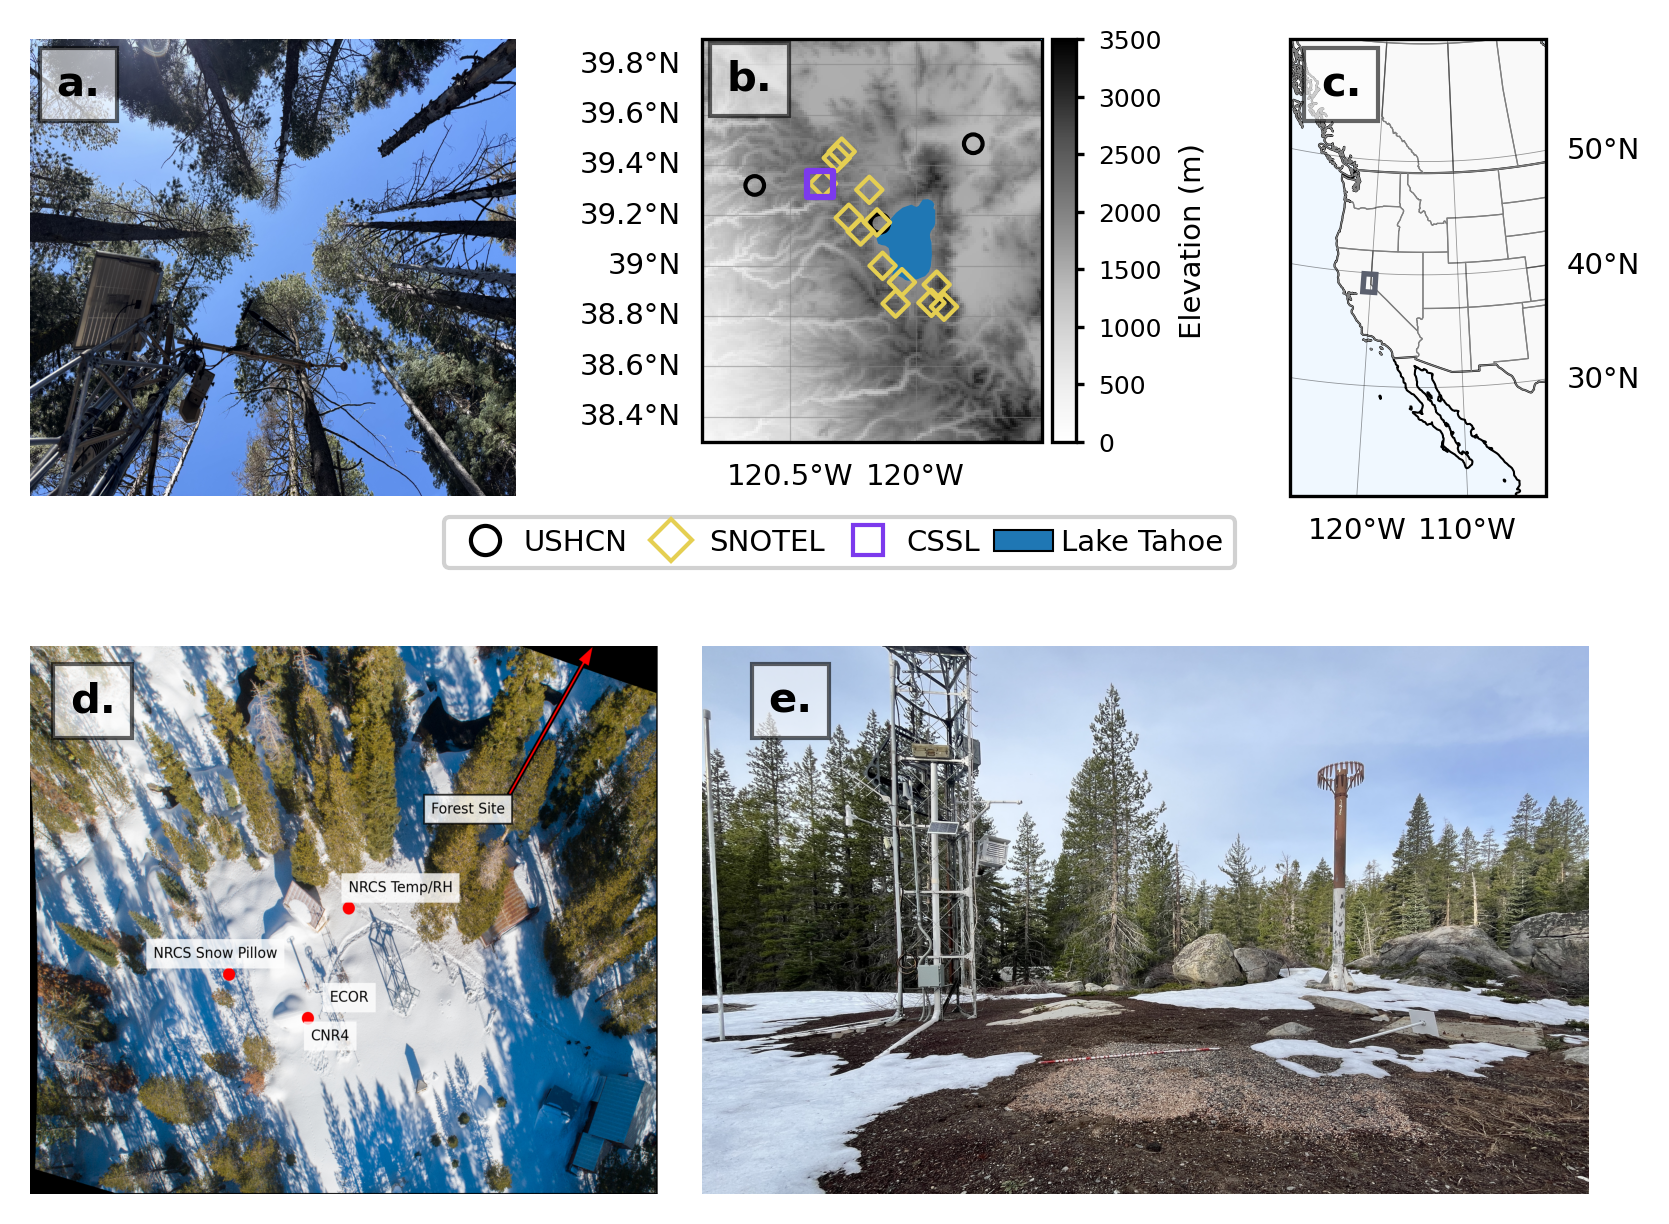
\includegraphics[width=\linewidth]{images2/region_map.png}
  \caption{
  The California Sierra Nevada study region.
  (a) An up-looking view from the forest site at CSSL. 
  (b) Terrain elevation of the greater CSSL/Lake Tahoe region. 
    Open diamonds depict the location of NRCS SNOTEL sites, open circles show the location of the four USHCN stations in the region, and the open purple square shows the location of CSSL.
  (c) Shows the location of the study area in the context of the WUS, with the boundary of (b) outlined by an open rectangle.  
  (d) Shows an overview aerial image of CSSL open site, with key instruments labeled, including the ECOR (eddy covariance).
  The forest study site is just outside of the frame to the top right.
  (e) Depicts the NRCS snow pillow (and precipitation bucket in the background) at CSSL on March 30, 2026.
  }
  \label{fig:region_map}
\end{figure}


% USHCRN data
\begin{figure}[htbp]
  \centering
  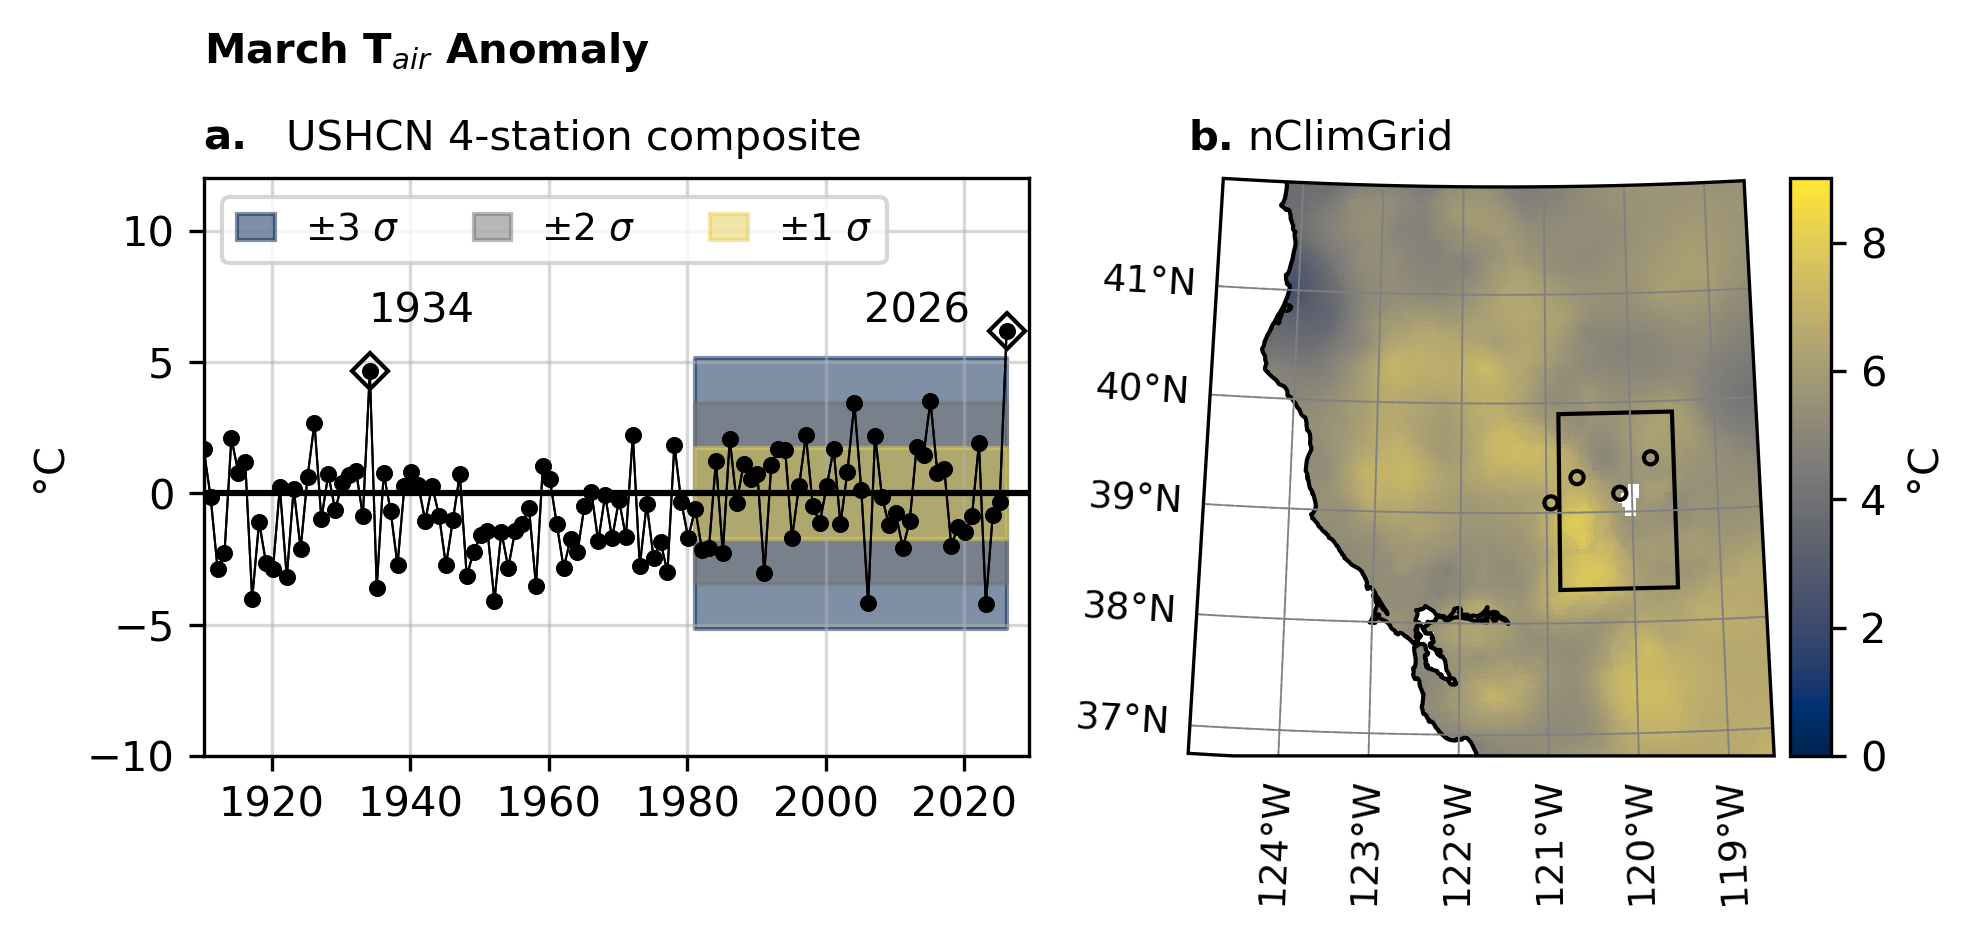
\includegraphics{images2/temp_anomaly_map.png}
  \caption{(a) Composite \tair anomalies from the four HCNv2 dataset stations in the greater central California Sierra Nevada region study area for the month of March, from 1910 to 2026. 
  Deviations and standard deviations with respect to the 1981--2010 mean \tair are depicted using shading. 
  (b) The same, but for a map-view of the \tair anomaly of the gridded nClimGrid product.
  The box depicts the map boundary from \fig{fig:region_map}{b} and open circles depict USHCN station locations.
  }
  \label{fig:ushcn_data}
\end{figure}


% ERA5 data
\begin{figure}[htbp]
  \centering
  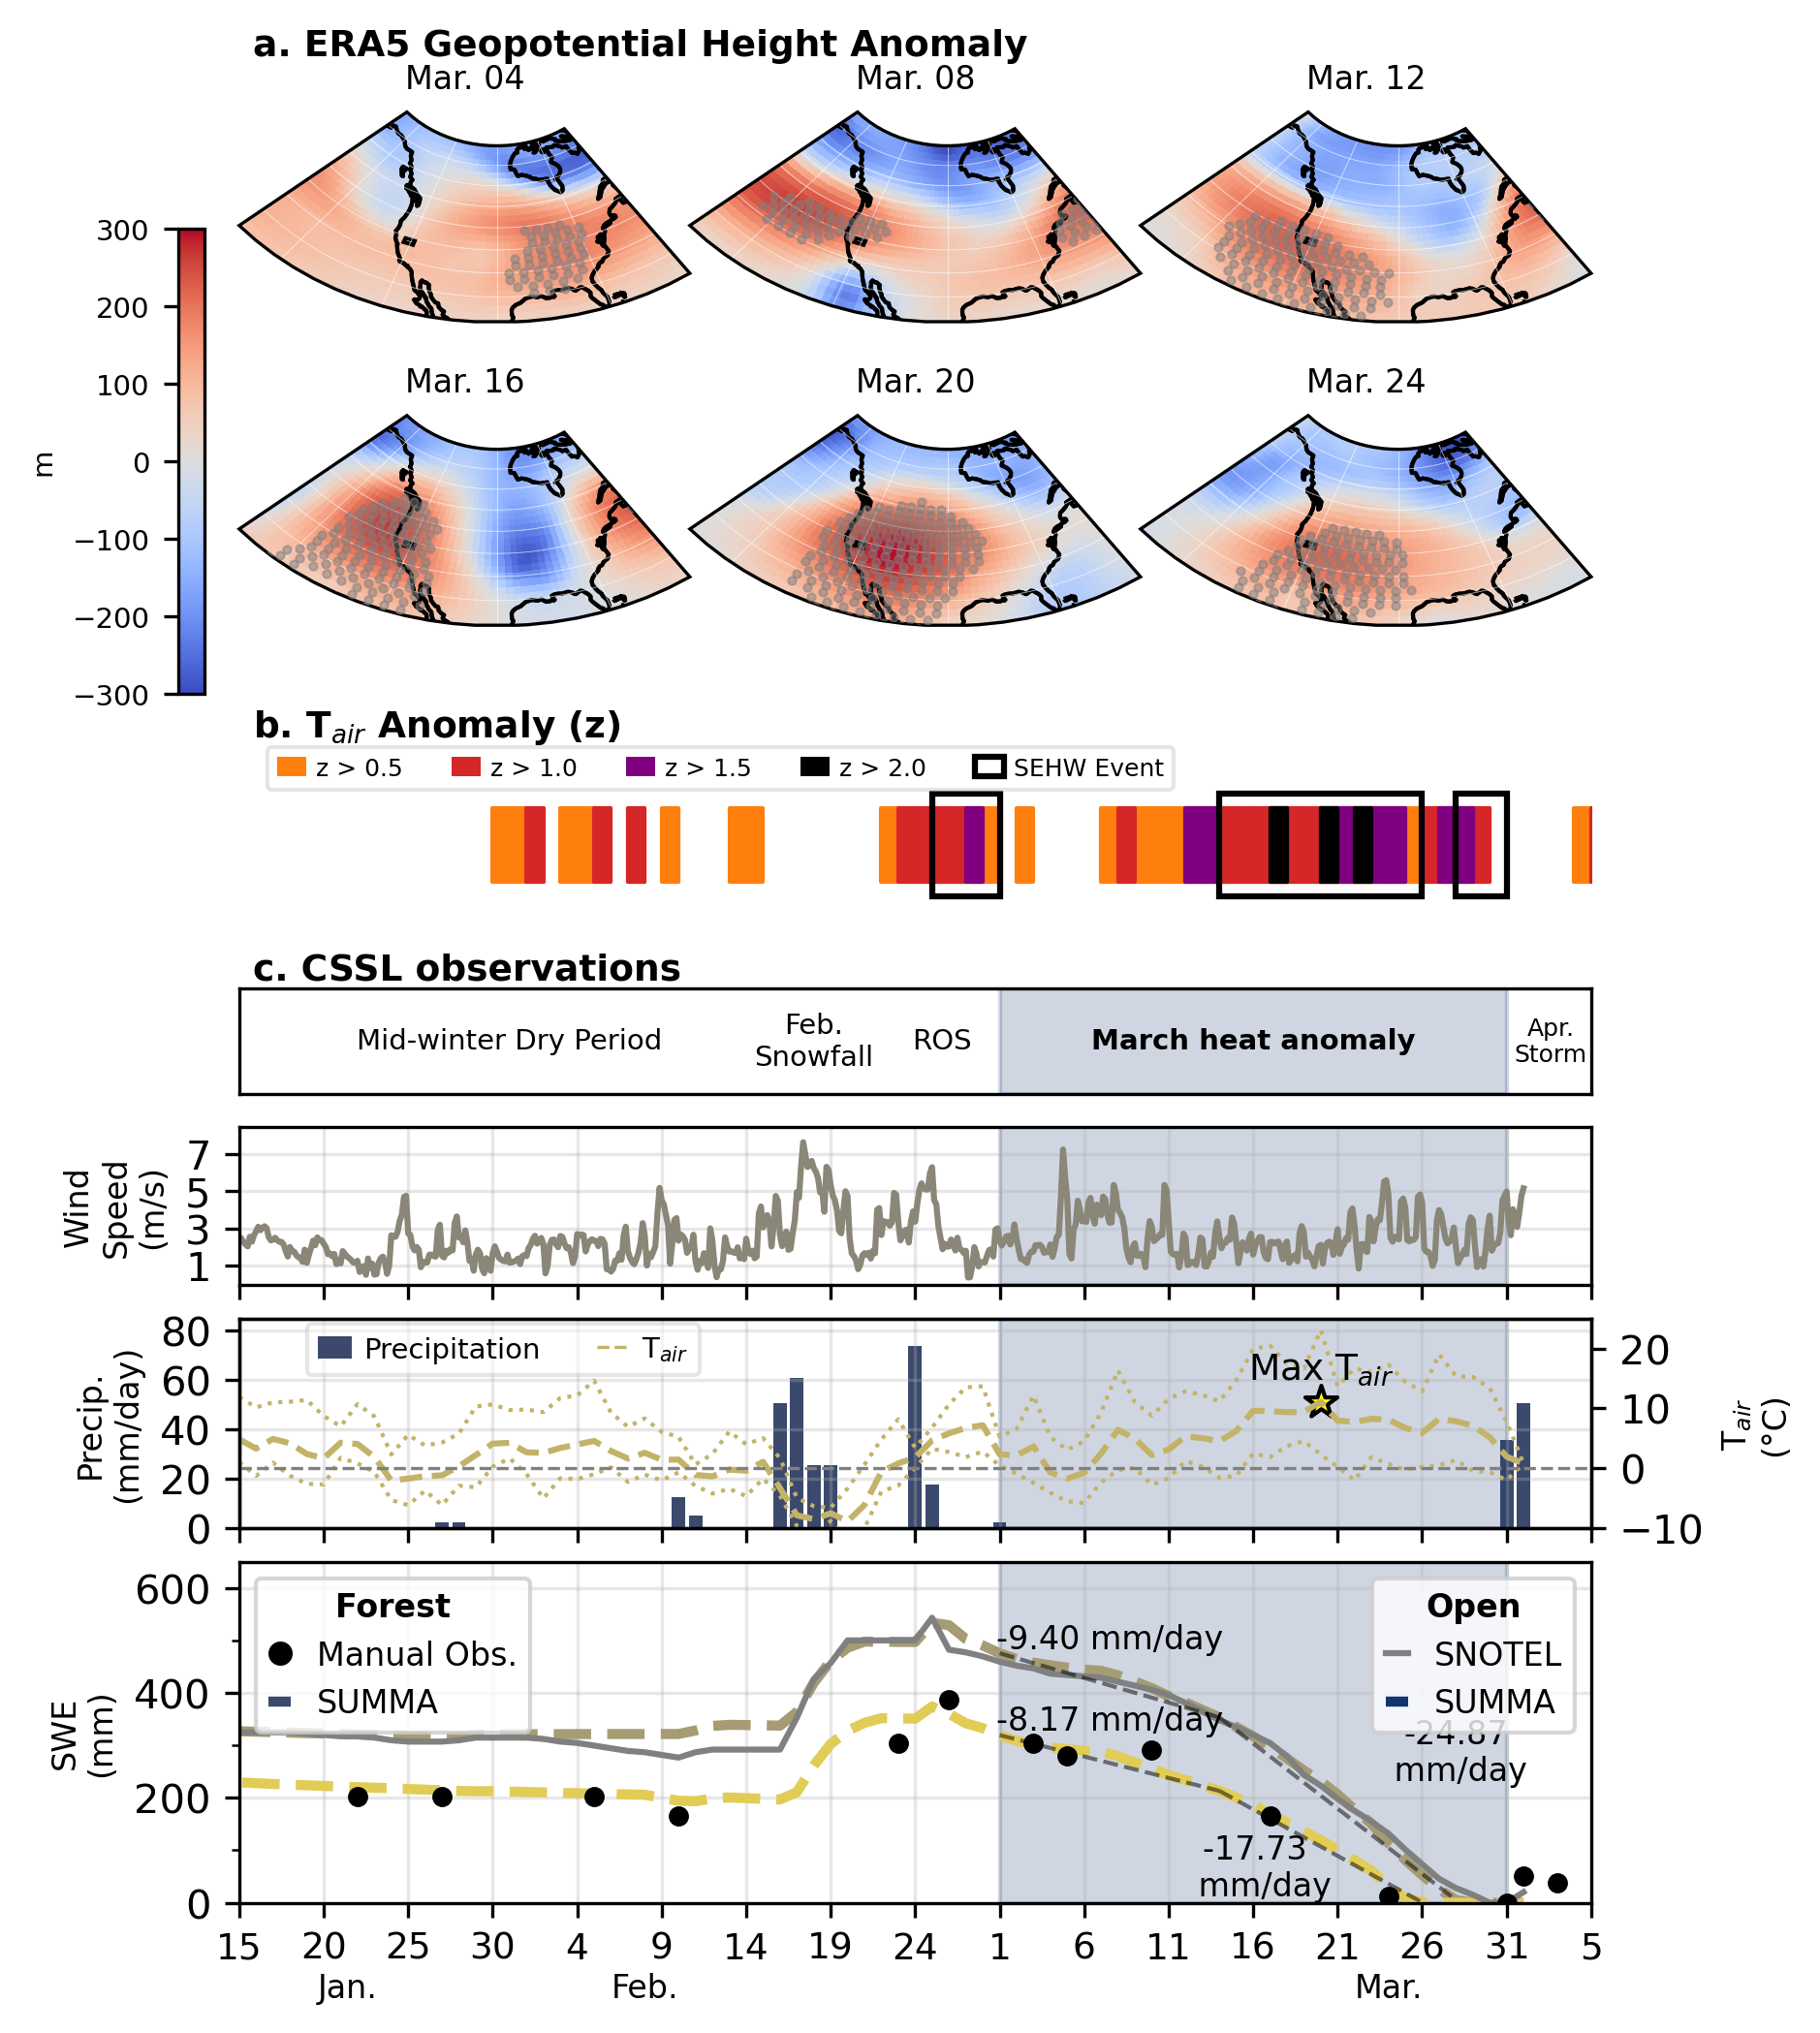
\includegraphics[width=\linewidth]{images2/mar2026_era5_snotel_summary.png}
  \caption{
  (a) The 500 hPa geopotential height anomaly during March 2026 heat wave from ERA5 across the WUS for six individual days.
  The study region is outlined using an overlain black rectangle.
  Gray stippling indicates regions with 500 hPa geopotential height anomalies greater than 2-$\sigma$ above the March mean.
  (b) depicts two meter \tair anomaly z-scores from the Tahoe City USHCN station. 
  Periods meeting the \citeA{Rhoades2026-jm} SEHW criteria are outlined with a black box. 
  (c) shows the time series of meteorological and snow conditions at CSSL, with different synoptic conditions highlighted by background shading (top-panel).
  Wind speed, precipitation, and two-meter \tair are depicted (daily average, daily minimum, and daily maximum). 
  The bottom panel depicts modeled (SUMMA) and observed SWE at the open and forest sites. 
  Average rates of SWE loss are listed in the figure text with dashed lines superimposed on the SWE curves.
  }
  \label{fig:era5_anoms}
\end{figure}


\begin{figure}[htbp]
  \centering
  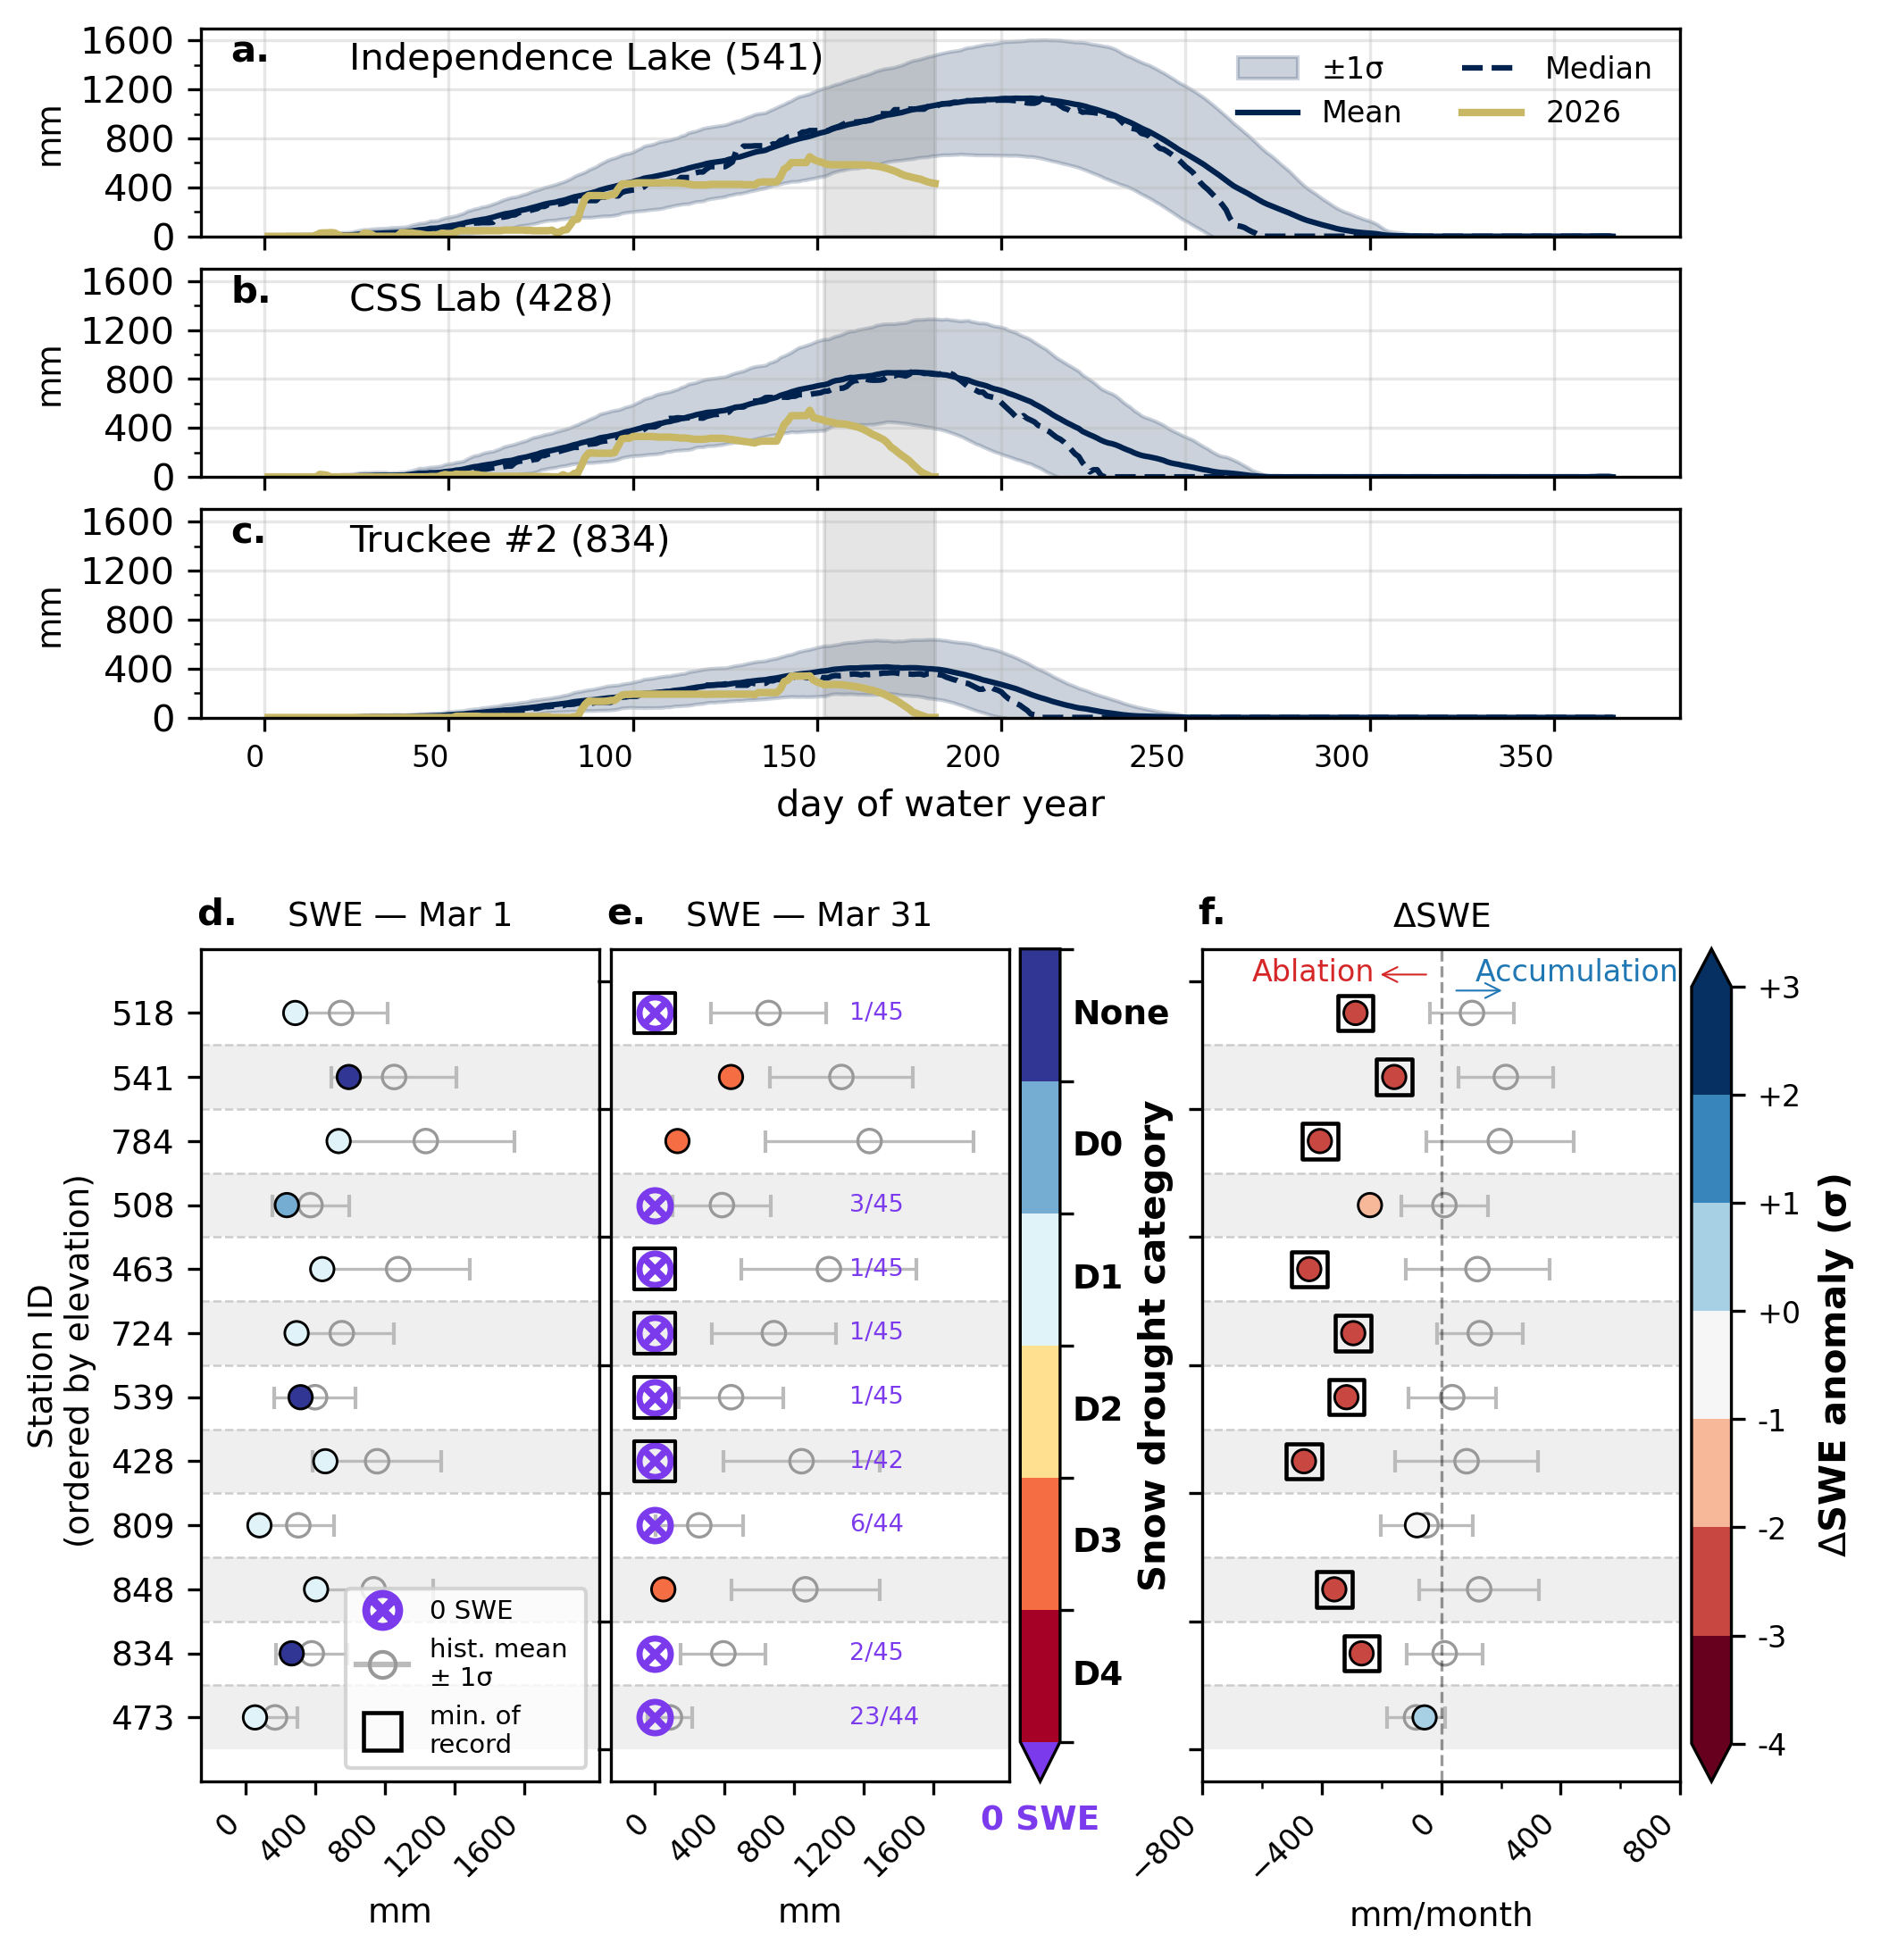
\includegraphics[width=\linewidth]{images2/swe_change_2026_v2.png}
  \caption{(a--c) Timeseries of SWE at three SNOTEL stations in the study region.
  The mean, median (dashed line), 1-$\sigma$ (shaded region) and water year 2026 values are depicted.
  (d) SWE values on March 1st for the 12 SNOTEL sites in the study domain, labeled by their three-digit station code.
  (e) The same as (d), but for SWE on March 31.
  Color values depict the \citeA{Hatchett2022} snow drought category.
  A 0 mm of SWE value is depicted by a purple circle marker.
  The purple text lists the number of 0 mm SWE occurrences observed on that date relative to the period of record for that site.
  (f) The SWE change between Mar 31 and Mar 1 (\dswe) compared with the historical record.
  Color values depict the deviation from the mean in units of $\sigma$.
  Square markers bounding symbols indicate that the SWE or \dswe is the record minimum for the period of record.}
\label{fig:swechange}
\end{figure}



\begin{figure}[htbp]
  \centering
  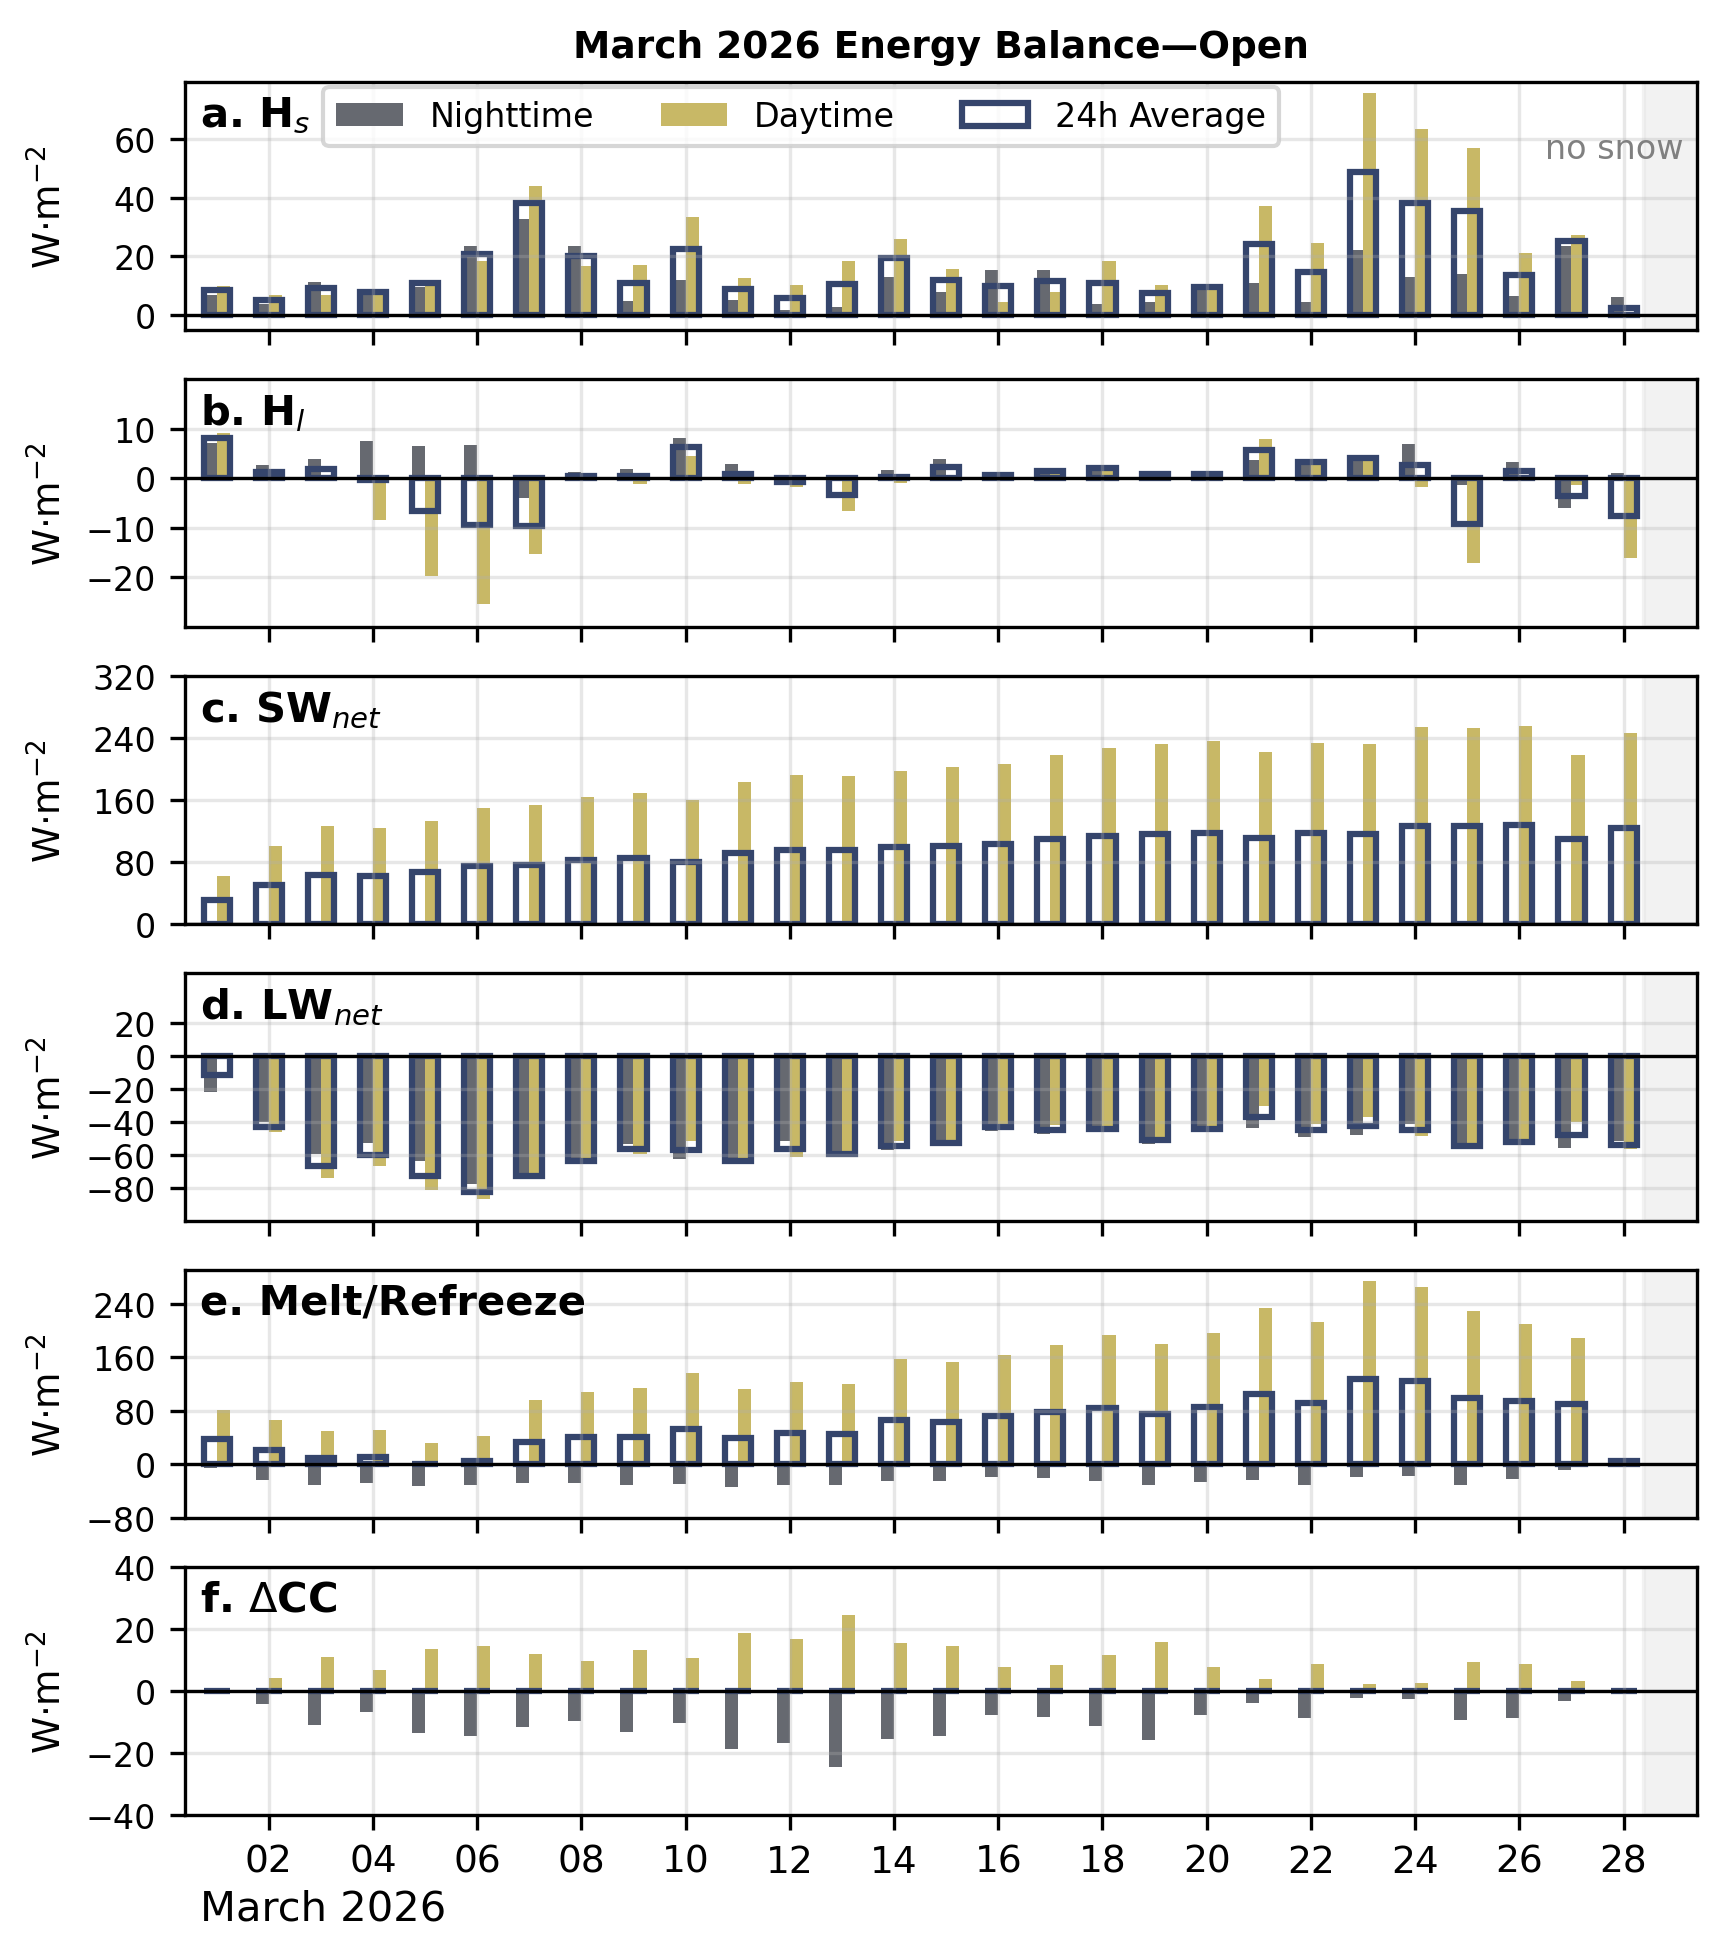
\includegraphics[width=\linewidth]{images2/mar_seb_open.png}
  \caption{Daily average energy flux components including (a) $H_s$, (b) $H_l$, (c) \swnet, (d) \lwnet, (e) snowpack Melt/Refreeze and (f) change in CC ($\Delta$CC) during the March 2026 heat wave at the open site.
  Each day has three bars: the left-most yellow bar depicts the daytime flux, the right-most gray bar depicts the nighttime flux, and the outline spanning both bars depicts the 24-hour average flux.
  Note that the y-scales are not equivalent across all of the figures.
  }
  \label{fig:open_seb}
\end{figure}



\begin{figure}[htbp]
  \centering
  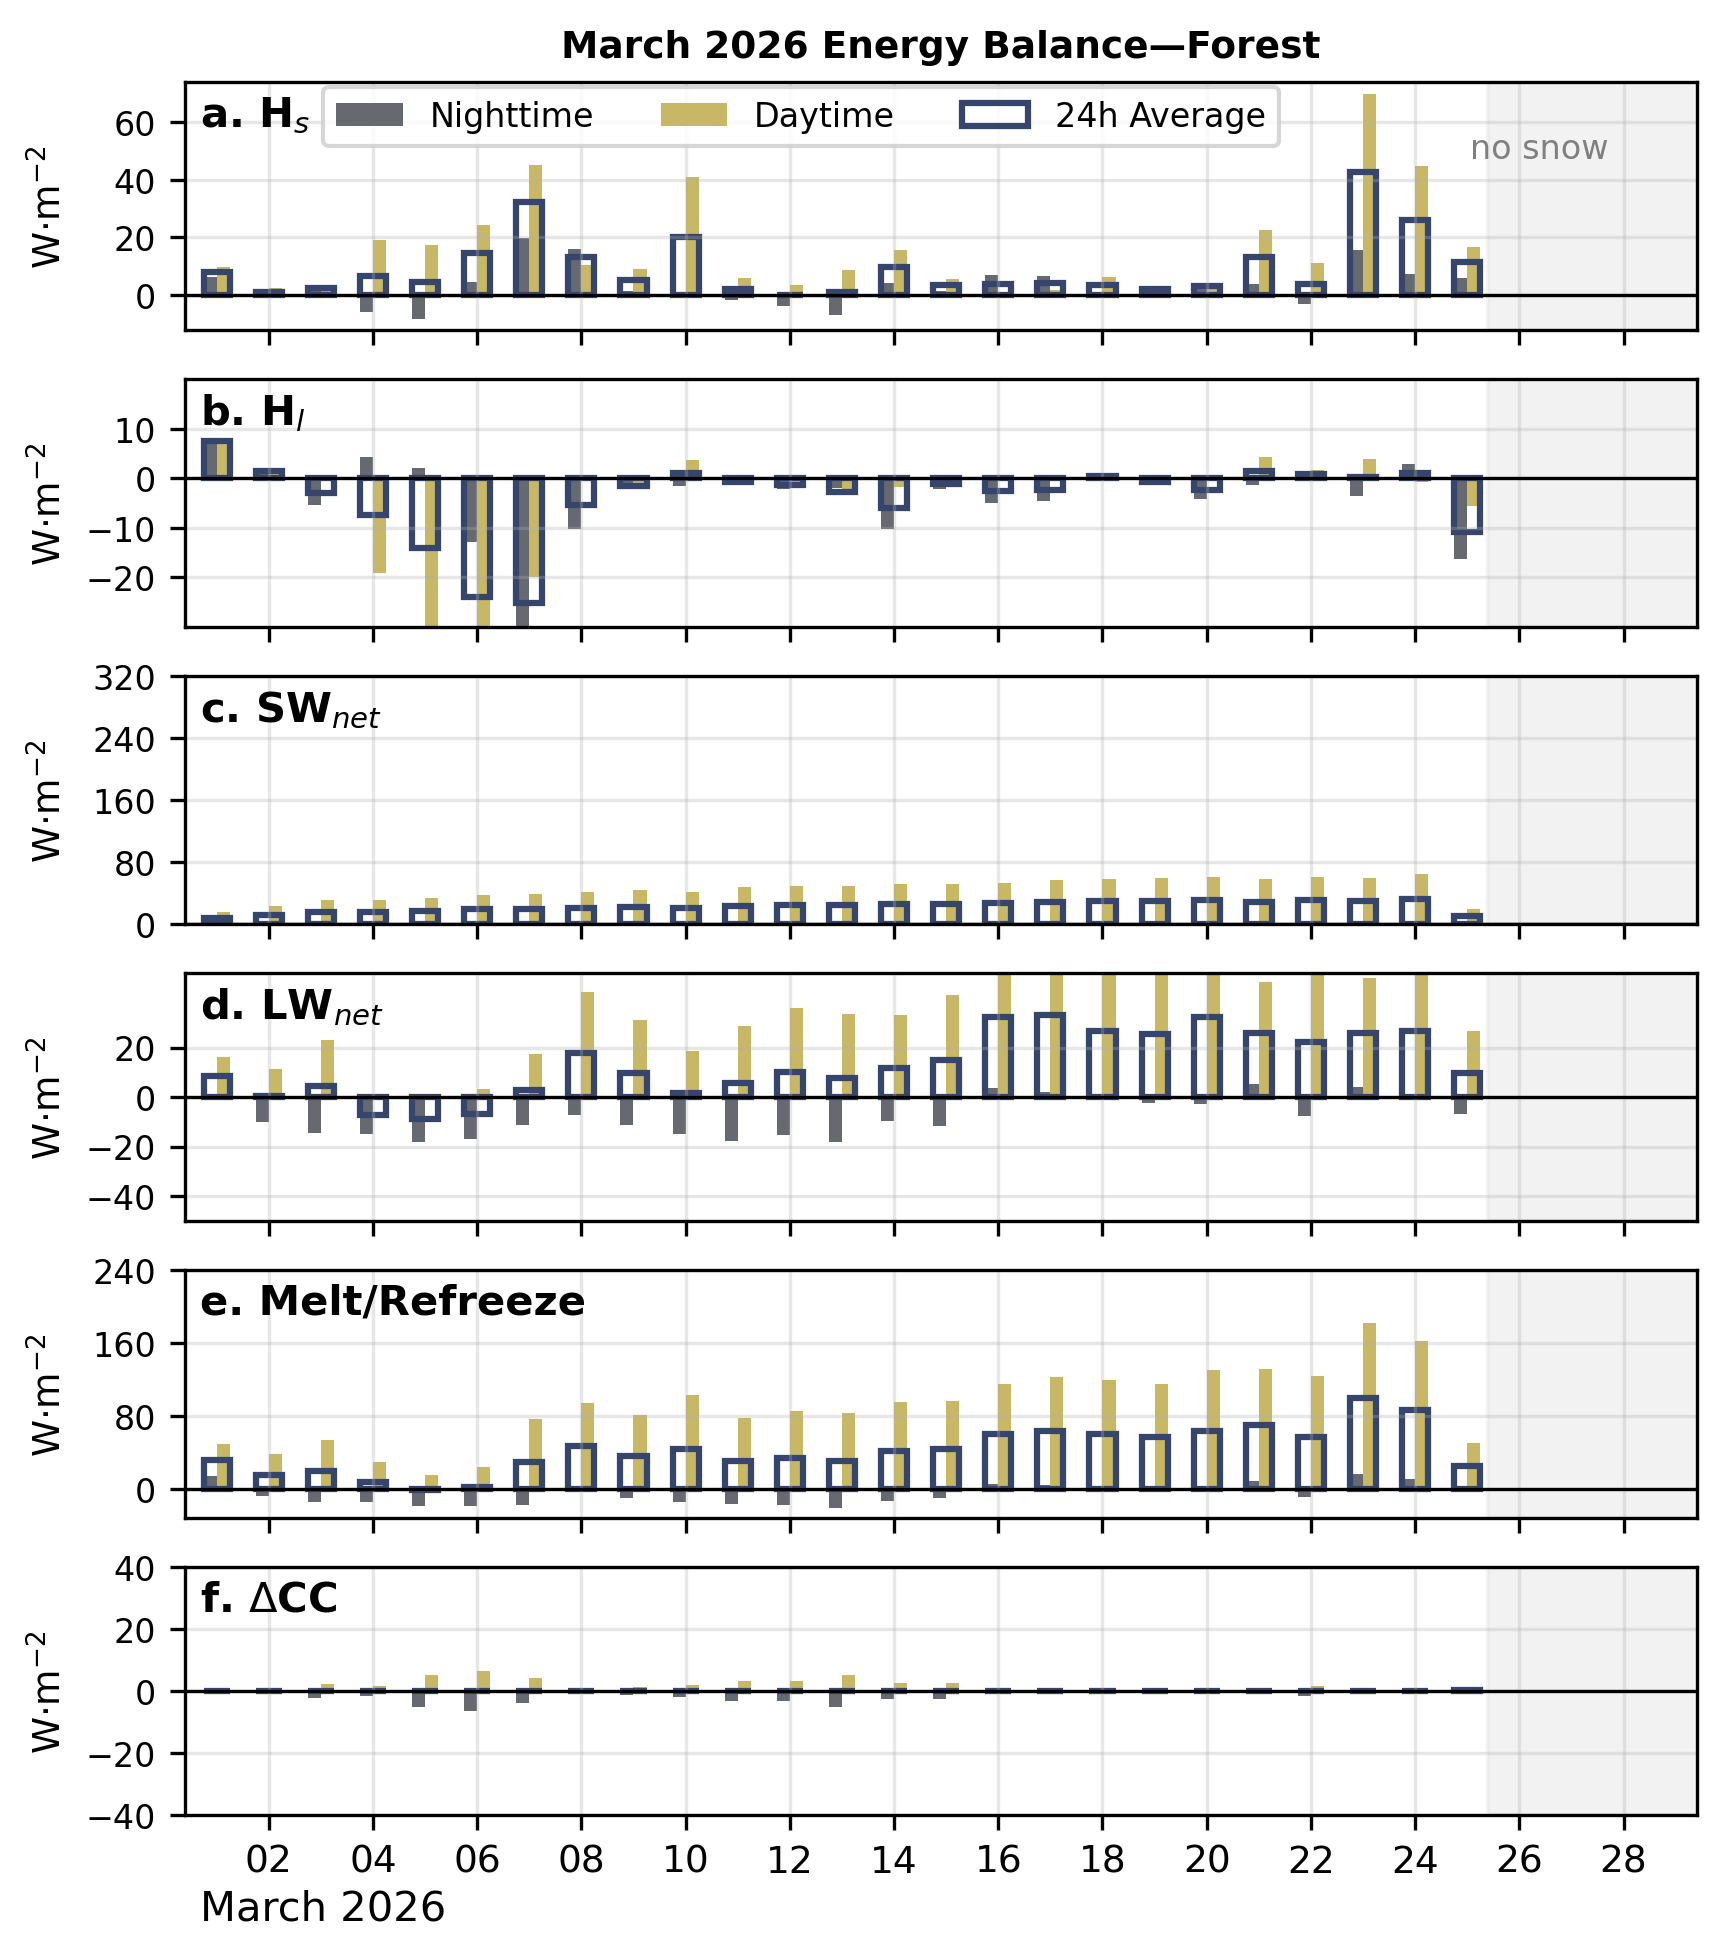
\includegraphics[width=\linewidth]{images2/lai_p5_seb.png}
  \caption{The same as \fignop{fig:open_seb}{} but for the forest site.
   Note that the y-axis limits and ticks are not the same as \fignop{fig:open_seb}{}.}
  \label{fig:forest_seb}
\end{figure}


\begin{figure}[htbp]
  \centering
  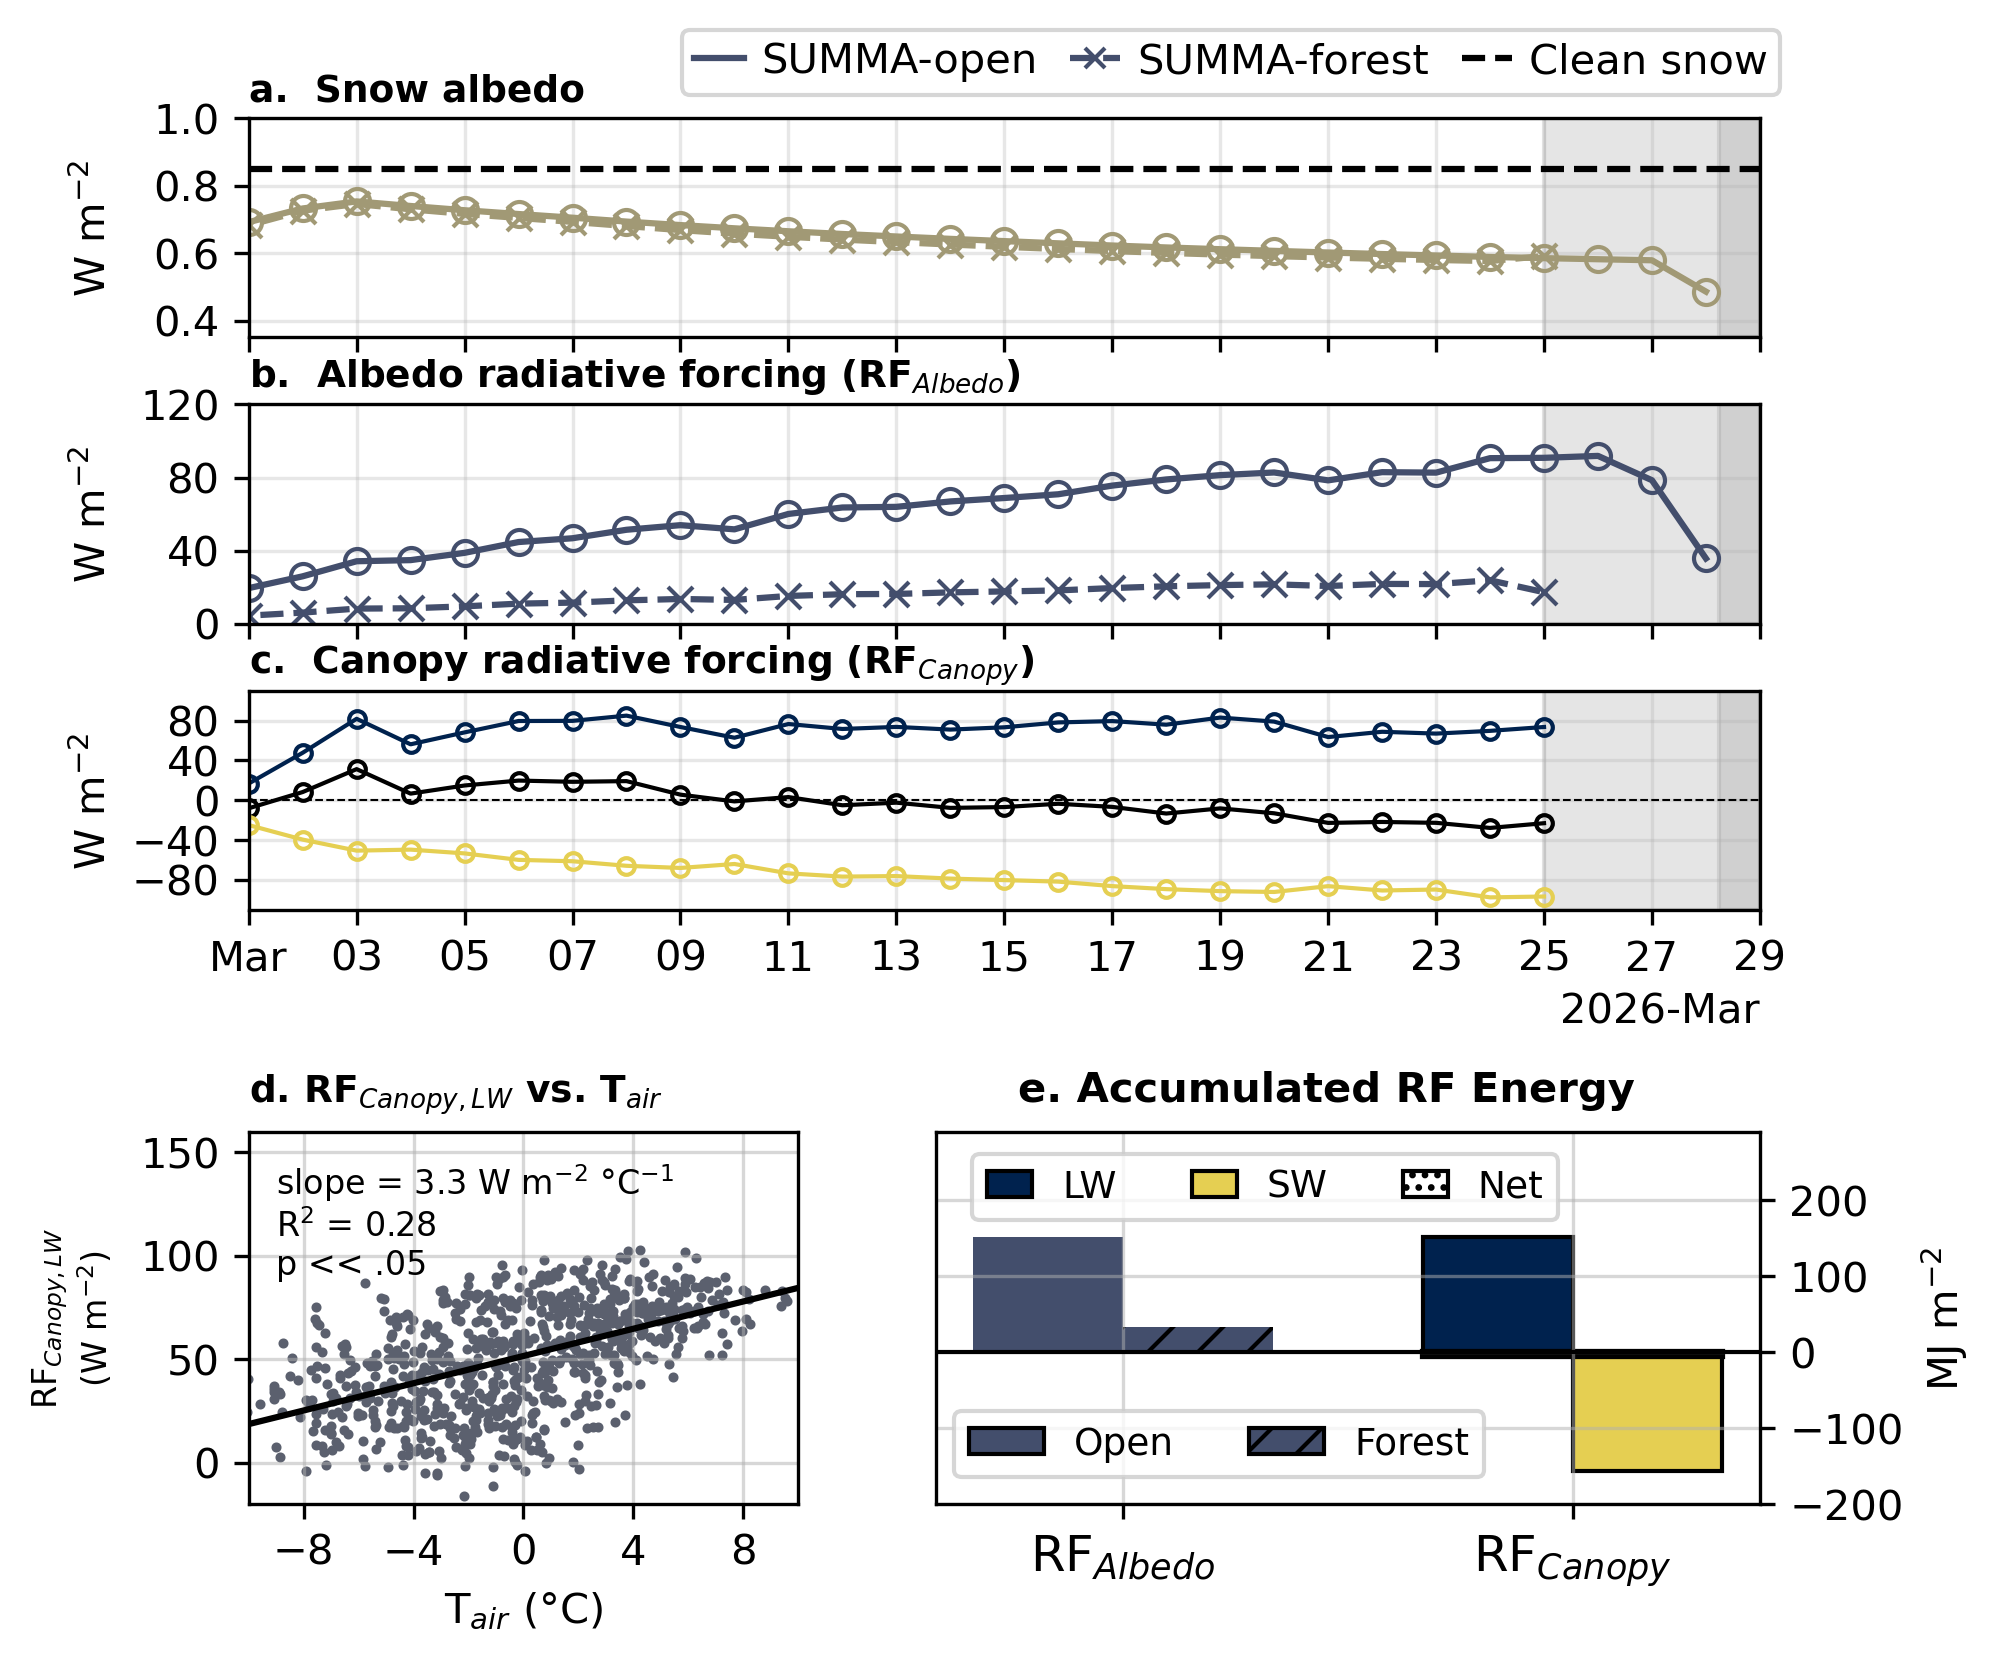
\includegraphics[width=\linewidth]{images2/canopy_lw_radiation_effect_and_albedo.png}
  \caption{Timeseries of (a) \albedo, (b) \rfalb, (c) \rfcanopy for March 2026. 
  The LW, SW, and net (LW + SW) components are all depicted in (c).
  (e) Depicts the relationship between daily-average \tair and the LW component of \rfcanopy for all Marches in the SUMMA historical record (2000--2026).
  (f) Depicts accumulated energy terms during the snow-covered duration of March.
  The stippled net \rfcanopy is negative but too small to resolve on the plot. 
  }

  \label{fig:radiative_forcing}
\end{figure}


\begin{figure}[htbp]
  \centering
  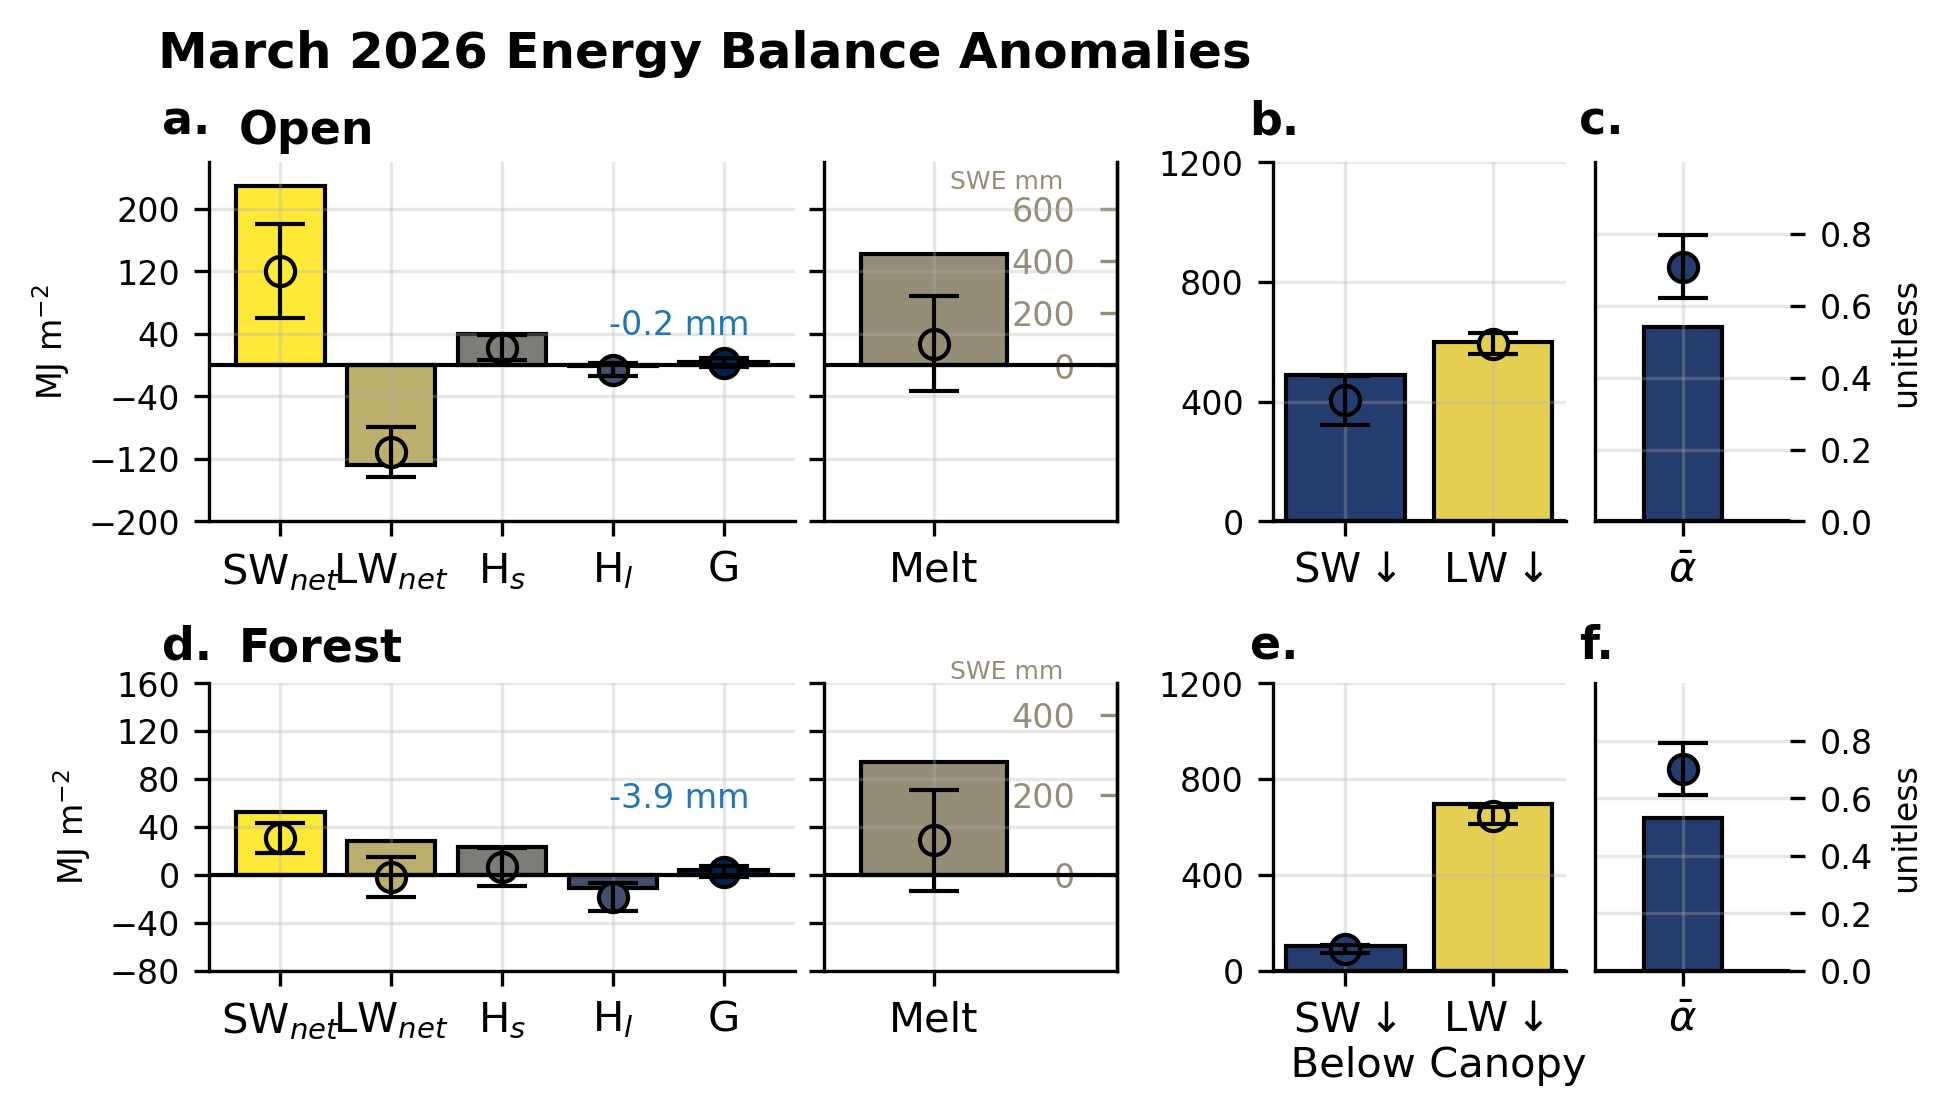
\includegraphics{images2/mar_seb_open_v_forest.png}
\caption{Accumulated snow energy fluxes (\swnet, \lwnet, \hs, \hlat, G), Melt, radiation forcings,
(\swdn, \lwdn), and weighted snow $\bar{\alpha}$ for the open (a--c) and forest (d--f) sites for the duration of March 2026, restricted to times when SWE is present.
Open circles and whiskers show the average and 1-$\sigma$ from the March SUMMA historical period (2000--2026).
Equivalent units of mm of melt are displayed in red text on the right-hand side of the Melt panels (a and d).
The under-canopy \swdn and \lwdn are depicted in panel (e).
}\label{fig:monthly_seb_mar}
\end{figure}


\begin{figure}[htbp]
  \centering
  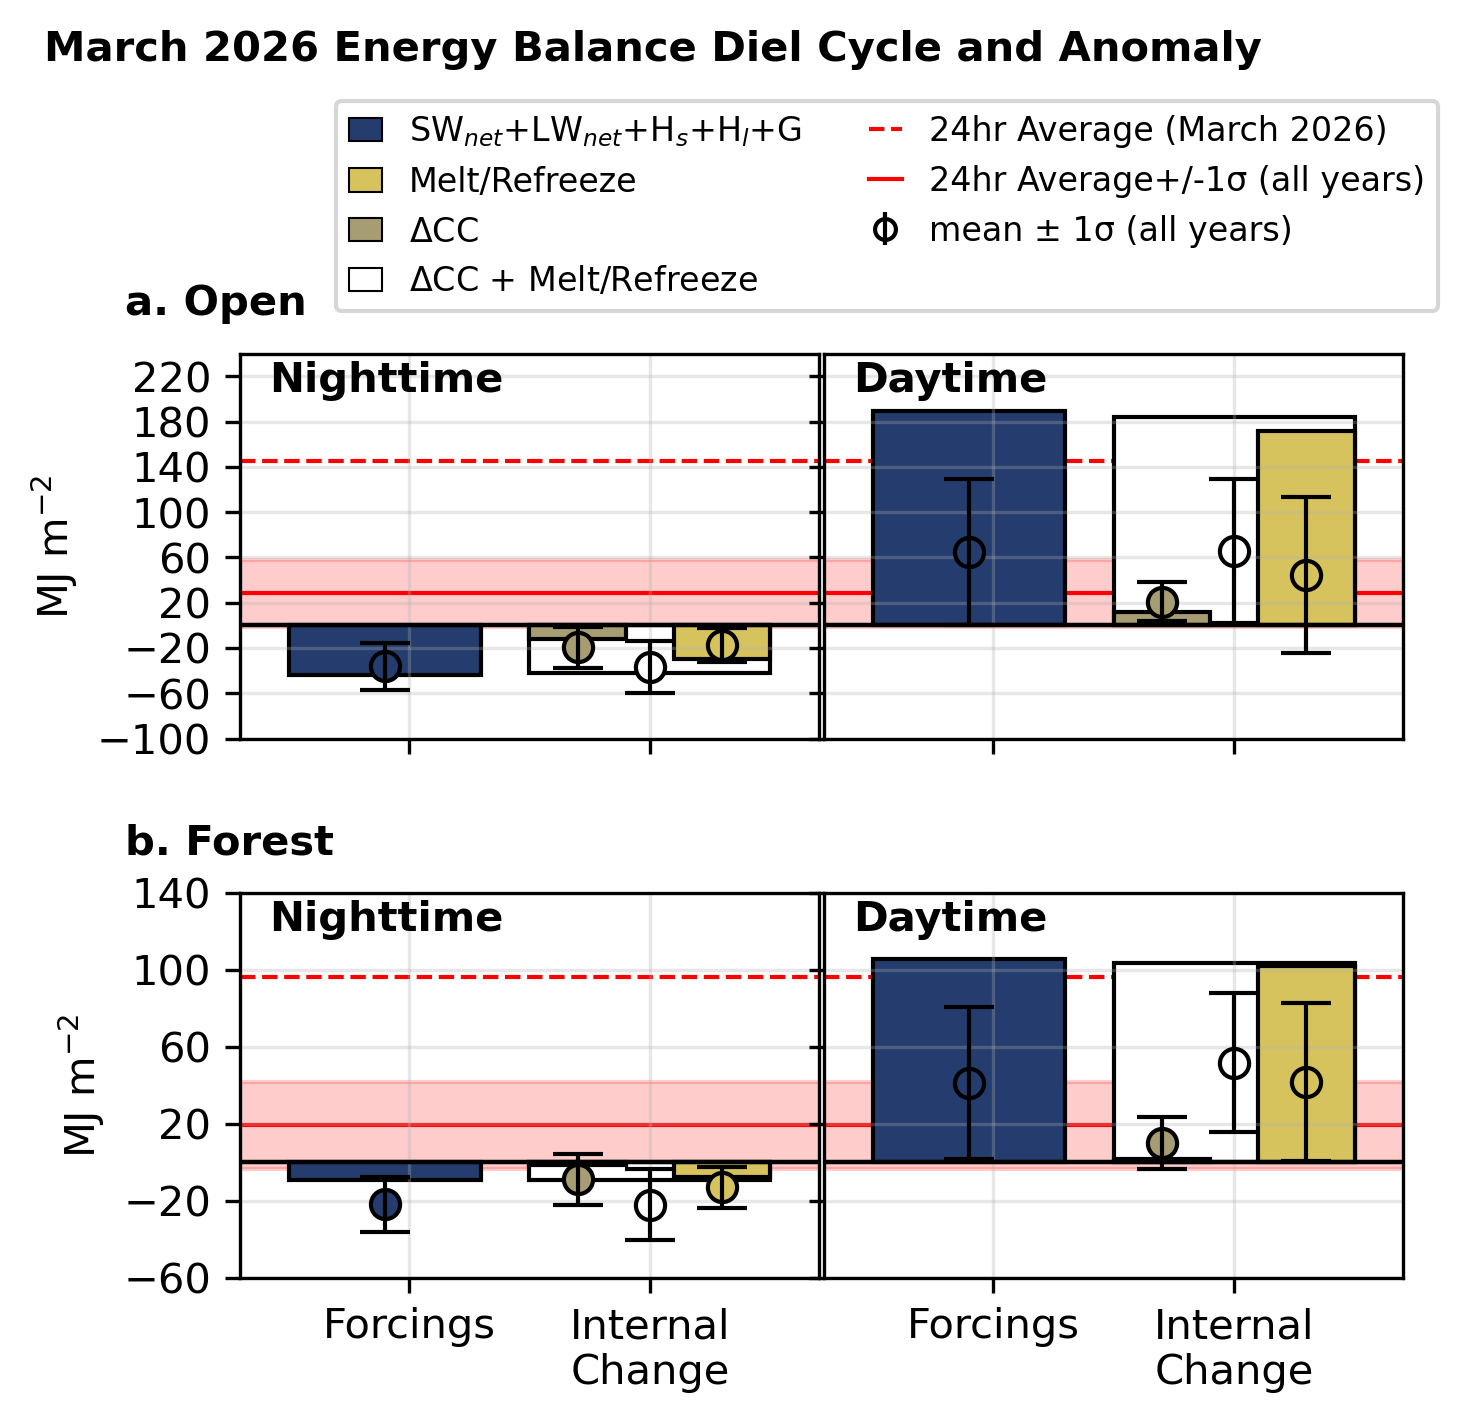
\includegraphics[width=\linewidth]{images2/mar_diel_seb_open_v_forest.png}
  \caption{Similar to Fig. \ref{fig:monthly_seb_mar}, but for daytime, nighttime, and 24-hour sums of accumulated energy balance components in the (a) Open and (b) Forest sites.
  Forcings include net-radiative and turbulent flux terms at top and bottom boundaries of the snowpack.
  Internal Change terms are the accumulated \dcc and melt (positive) and refreezing (negative) energy.
  $\Delta$CC and Melt/Refreeze are separated into individual terms for visualization purposes.
  }
  \label{fig:mar_diel_seb_open_v_forest}
\end{figure}


\begin{figure}[htbp]
  \centering
  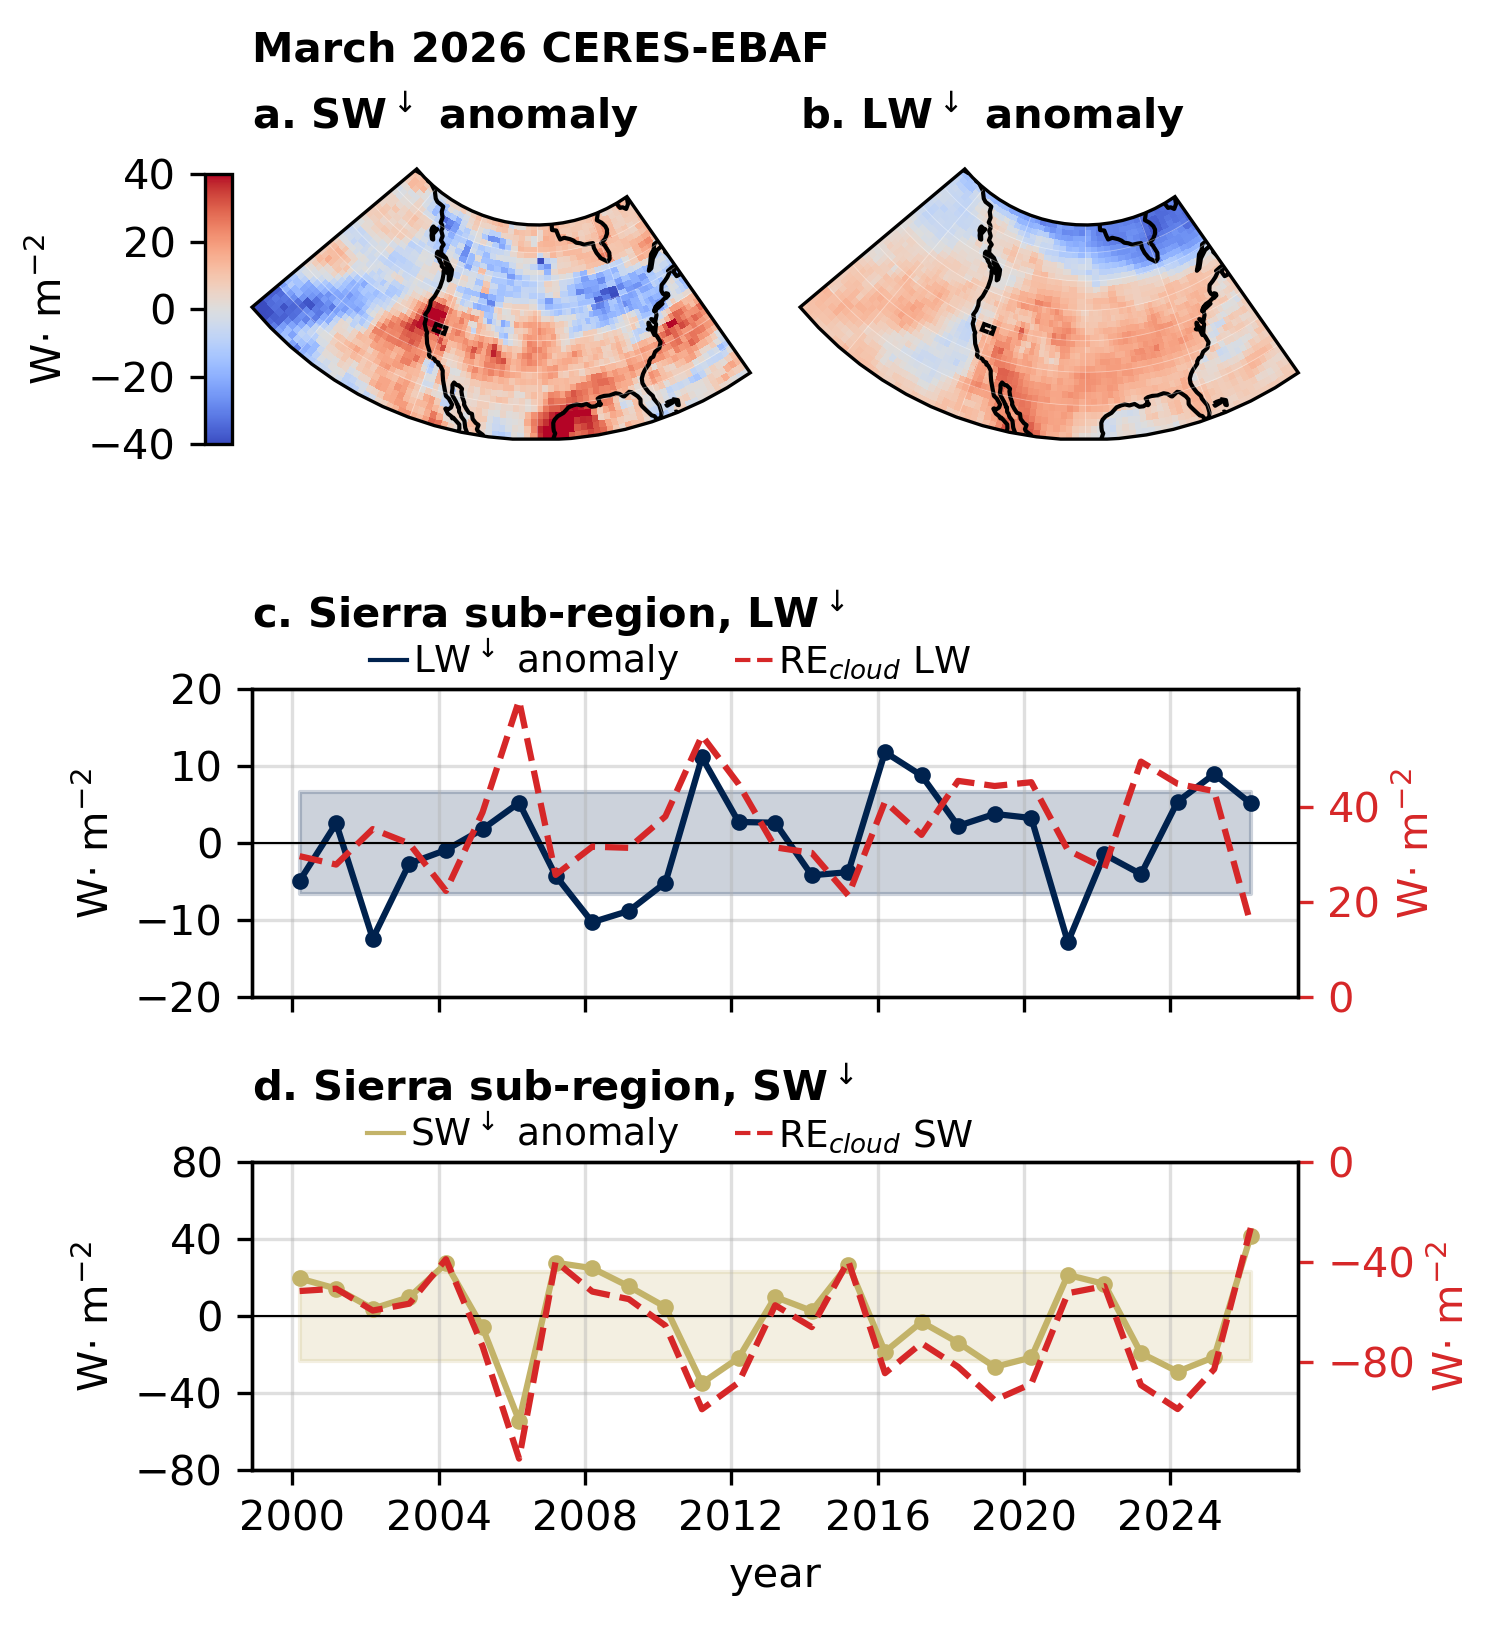
\includegraphics{images2/ceres_ebaf_anomaly.png}
  \caption{March \swdn (a) and \lwdn (b) anomalies (relative to the March 2000 to present record) from the CERES-EBAF 1$^\circ\times$1$^\circ$ resolution product.
  (c) and (d) depict the timeseries of anomalies averaged over the Sierra Nevada study region.
  RE$_{cloud}$ amount is depicted with a twin y-axis, with units displayed on the right-hand side in red text.
  The shaded region in each plot depicts 1-$\sigma$ of the anomaly.
  }
  \label{fig:ebaf_anomaly}
\end{figure}


\begin{figure}[htbp]
  \centering
  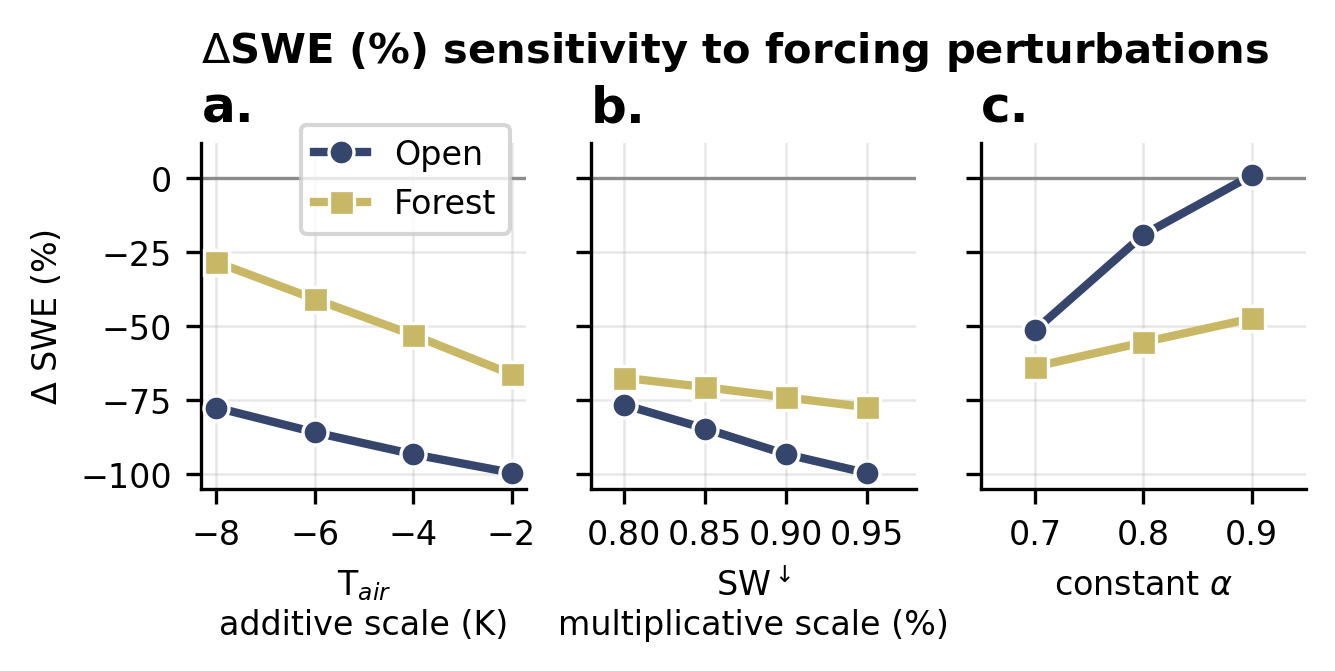
\includegraphics{images2/swe_pct_change_forest_vs_open_frc_sens.png}
  \caption{Sensitivity of \dswe (\%) from March 1 to March 31 to perturbations to (a) \tair and (b) \swdn forcings for open and forest sites.
  (c) shows the effect of prescribing a constant broadband snow \albedo.}
  \label{fig:idealized_sensitivity}
\end{figure}



\begin{figure}[htbp]
  \centering
  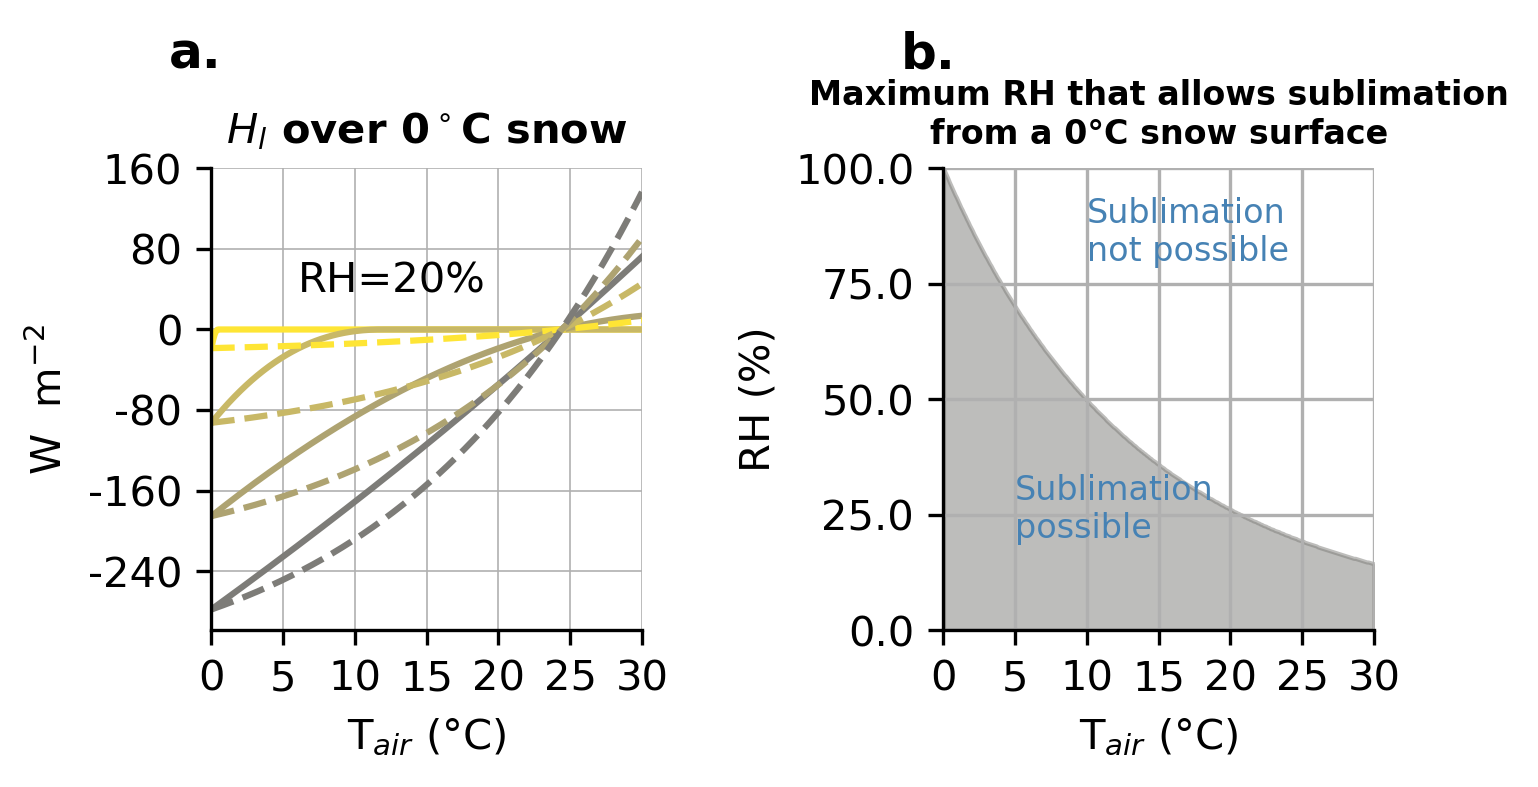
\includegraphics{images2/idealized_sens_and_lat_heat.png}
  \caption{
  (a) Idealized latent heat fluxes ($H_l$) into a melting snowpack as a function of \tair for four wind speeds (1, 5, 10, and 15 m s$^{-1}$) at a 12 m height for open-conditions and a snow surface roughness of z$_0$=0.002 m.
  Dashed lines show flux assuming a neutral surface layer; solid lines show the same formulation with a stability correction applied.
  Contours depict the fraction of the maximum $H_s$ for that wind speed value.
  (b) The thermodynamic limitation of sublimation as a function of \tair, depicting the maximum RH that permits sublimation from a 0 \degrc snowpack.
  }
  \label{fig:idealized_sens_heat}
\end{figure}





\clearpage


%%% WHOLE MONTH TABLE 
\begin{table}[h]
\centering
\caption{Open and forest-site energy balance terms (\mjmtwo; mm SWE equivalent in parentheses for H$_l$ and Melt) and cold content change (\mjmtwo) for March 2026 compared against the historical climatology (mean $\pm$ std).}
\label{tab:forest_open_summary}
\begin{tabular}{llrrrrrrr}
\toprule
 & & SW$_{net}$ & LW$_{net}$ & H$_s$ & H$_l$ & G & Melt & $\Delta$CC \\
\midrule
\multirow{3}{*}{Open}   & 2026 & 229.3 & -127.5 & 39.7 & -0.7 (-0.2) & 4.3 & 142.1 (425.6) & 0.0 \\
 & Mean & 120.3 & -111.3 & 22.7 & -5.8 (-2.1) & 3.3 & 27.6 (82.6) & 1.8 \\
 & Std. & 61.3 & 32.8 & 16.0 & 8.6 (3.0) & 5.8 & 61.9 (185.4) & 4.8 \\
\midrule
\multirow{3}{*}{Forest} & 2026 & 52.1 & 28.1 & 22.9 & -11.0 (-3.9) & 4.0 & 94.3 (282.4) & 0.0 \\
 & Mean & 31.0 & -1.6 & 6.3 & -18.8 (-6.6) & 2.4 & 28.8 (86.2) & 1.0 \\
 & Std. & 12.7 & 17.0 & 16.0 & 11.9 (4.2) & 4.6 & 42.8 (128.2) & 2.3 \\
\bottomrule
\end{tabular}
\end{table}


\begin{table}[h]
\centering
\caption{Day/nighttime decomposition of Forcings (SW$_{net}$+LW$_{net}$+H$_s$+H$_l$+G), Melt/Refreeze, and $\Delta$CC, in \mjmtwo, for March 2026 compared against the historical climatology (mean $\pm$ std) of March conditions.}
\label{tab:forest_open_diel_summary}
\begin{tabular}{llrrrrrr}
\toprule
 & & \multicolumn{2}{c}{Forcings} & \multicolumn{2}{c}{Melt/Refreeze} & \multicolumn{2}{c}{$\Delta$CC} \\
\cmidrule(lr){3-4} \cmidrule(lr){5-6} \cmidrule(lr){7-8}
 & & Day & Night & Day & Night & Day & Night \\
\midrule
\multirow{3}{*}{Open}   & 2026 & 189.2 & -44.1 & 172.1 & -29.9 & 11.9 & -11.9 \\
 & Mean & 64.7 & -36.2 & 44.7 & -17.4 & 21.0 & -19.5 \\
 & Std. & 65.5 & 21.0 & 69.9 & 15.6 & 17.5 & 18.7 \\
\midrule
\multirow{3}{*}{Forest} & 2026 & 105.4 & -9.2 & 101.9 & -7.5 & 1.7 & -1.7 \\
 & Mean & 41.1 & -21.9 & 41.8 & -13.1 & 9.9 & -9.0 \\
 & Std. & 40.4 & 14.5 & 41.9 & 10.7 & 13.8 & 13.4 \\ 
\bottomrule
\end{tabular}
\end{table}




%%% DAY AND NIGHT TABLE 
\begin{table}[h]
\centering
\caption{Definitions used in this study.}
\label{tab:definitions}
\begin{tabular}{ll}
\toprule
Abbreviation & Definition \\
\midrule
CSSL         & Central Sierra Snow Laboratory \\
CERES-EBAF   & Clouds and the Earth's Radiant Energy System Energy Balanced and Filled product \\
SNOTEL       & SNOwpack TELemetry site \\
SEHW         & Snow-eater heat wave \\
SUMMA        & Structure for Unifying Multiple Modeling Alternatives \\
USHCN        & US Historical Climatology Network \\
WUS          & Western United States \\
\bottomrule
\end{tabular}
\end{table}




\clearpage

% --- BIBLIOGRAPHY ---
% \bibliographystyle is set to apacite by agujournal2019.cls
\bibliography{paperpile} % Ensure paperpile.bib is in the same folder
\end{document}
